\documentclass{jfm}

% Compilation
\usepackage{silence} % Silence latex compiler warnings
\WarningFilter{latex}{Command \@xhline has changed} % Filter out warning
  % caused by redefinition between jfm.cls class and array (loaded by
  % siunitx)

% Import custom style file containing common packages and options
\setlength{\paperheight}{\pdfpageheight} % JFM class removes paperheight definition and hyperref raises a warning

\usepackage[section]{placeins} % force floats to appear in their subsection
\let\Oldsection\section
\renewcommand{\section}{\FloatBarrier\Oldsection}
\let\Oldsubsection\subsection
\renewcommand{\subsection}{\FloatBarrier\Oldsubsection}
\let\Oldsubsubsection\subsubsection
\renewcommand{\subsubsection}{\FloatBarrier\Oldsubsubsection}

% Import custom style file containing common packages and options
\usepackage{preamble}
\graphicspath{{./Figures/}}

% Discrete Fourier Transform
\newcommand{\GenP}{\hat{P}_m}
\newcommand{\POne}{\hat{P}_1}
\newcommand{\PTwo}{\hat{P}_2}
\newcommand{\PThree}{\hat{P}_3}
\newcommand{\PFour}{\hat{P}_4}

% Continuous Fourier Transform
\newcommand{\GenPk}{\hat{P}(\kappa)}
\newcommand{\PZerok}{\hat{P}(0)}

% Define custom math symbols
\DeclareMathOperator{\cn}{Cn}
\DeclareMathOperator{\sgn}{sgn}
\DeclareMathOperator{\Ur}{Ur}
\DeclareMathOperator{\Sk}{Sk}
\DeclareMathOperator{\As}{As}
%\DeclareMathOperator{\Bi}{Bi}

% Define \im as Roman i
\newcommand{\im}{\mathrm{i}}
% Replace epsilon with varepsilon
\renewcommand*{\epsilon}{\varepsilon}

%% Use \thalf and \squart commands from JFM class
%\newcommand\squart{\ensuremath{{\textstyle\frac{1}{4}}}}
%\newcommand\thalf{\ensuremath{{\textstyle\frac{1}{2}}}}

\title{Wind-Induced Changes to Surface Gravity Wave Shape in Shallow Water}

\author{Thomas J. Zdyrski \and Falk Feddersen}

\begin{document}

\maketitle

\begin{abstract}
Wave shape (e.g.,\ wave skewness and asymmetry) impacts sediment
transport, beach morphology, and ship safety.
Previous work by the authors showed that wind (via changes in surface
pressure) affects wave shape in intermediate and deep water.
This effect was most pronounced as the depth ($kh$) decreased.
Here, this work investigates the interaction of wind and wave shape in
shallow water.
A multiple-scales analysis is applied to waves propagating over a
shallow ($kh \ll 1$), flat bottom with a variety of wind-induced
surface-pressure profiles, such as Jeffreys-type and generalized
Miles-type.
The shallow depth enhances the influence of wind on wave shape and
intensifies the waves' second-harmonic modes.
The results are compared to previous wave-tank experimental data and
numerical simulation results.
\end{abstract}

\section{Introduction}
Directly comparing with \citet{feddersen2005wind} may be challenging
though; that experiment generated monochromatic, sinusoidal waves that
were subsequently forced by the wind.
However, since sinusoidal waves are not eigenfunctions of the KdV
equation, they will evolve (namely, energy will be passed to higher
harmonics even in the absence of wind).
Indeed, such a phenomena---in the unforced case---was observed over a
flat bottom by \citet{elgar1990recurrence,chapalain1992observed},
where the primary and first harmonic traded energy back and forth
periodically.
This same setup was treated numerically by \citet{liu2016modeling}
who also included the effects of wind.
The growth/decay of waves by wind was superimposed on this oscillation
amongst modes.

\Citet{liu2016modeling} also claim that this harmonic-oscillation
means that some downwind locations will measure virtually no skewness
or asymmetry, while others will.
They claim that this explains the observations of
\citet{feddersen2005wind}: the flat-bottomed portion of the tank saw
minimal effect of wind speed on skewness/asymmetry since it was located
at a node of this harmonic oscillation.
However, a wind-speed dependent change was observed on the sloping beach
portion since this measurement location was not a node.
Indeed, \citet{chapalain1992observed,liu2016modeling} observed these
oscillations to occur over \numrange{3}{4} wavelengths, and the
wave gauges of \citet{feddersen2005wind} were spaced \numrange{2}{3}
wavelengths apart, so this is consistent with one gauge being at a node
and the other at an antinode.
Note that this argument does not apply to the (pseudo-shallow water)
experiments by \citet{leykin1995asymmetry}: these waves were not
mechanically generated, but rather purely wind-generated.
Therefore, they do not necessarily begin as pure sinusoids and hence do
not suffer from these harmonic oscillations (likely being closer to
cnoidal waves, which do not experience such oscillations).

\section{Problem Solving Technique}
The governing equations are%
\footnote{
  We used the gauge freedom to absorb the Bernoulli ``constant'' $C(t)$
  in the dynamic boundary condition into the definition of $\phi$.
}
\begin{alignat}{2}
  0 &= \phi_{xx} + \phi_{yy} + \phi_{zz} &&\qq{on}
  -h < z < \eta \,, \label{eq:laplace}\\
  0 &= \phi_{z} &&\qq{on} z=-h \,, \label{eq:bottom_bc}\\
  \phi_{z} &= \eta_{t} + \phi_{x} \eta_{x} +
  \phi_{y} \eta_{y} &&\qq{on} z = \eta \,, \label{eq:kinematic_bc}\\
  \qq*{and} 0 &= \frac{p}{\rho_w} + g\eta + \phi_{t} +
  \frac{1}{2} \bqty{\phi_{x}^2 + \phi_{y}^2 + \phi_{z}^2} &&\qq{on} z=
  \eta \,. \label{eq:dynamic_bc}
\end{alignat}
We are seeking a quasi-periodic progressive wave of permanent form:
\begin{gather}
  \eta(\vec{x},t) = \eta(\theta, t) \qq{with} \theta \coloneqq
  \vec{x}\vdot\vec{k} - \omega t \,, \\
  \eta(\theta + 2\pi,t) = \eta(\theta,t) \,,
  \label{eq:periodicity_condition}
\end{gather}
with similar conditions on $\vec{u} \coloneqq \grad{\phi}$.
We are parameterizing our wave by four quantities: the depth, mean
Eulerian current, wave height, and wavelength.
We will use Stokes' first definition of wave celerity by taking the mean
current to be zero:
\begin{equation}
  \bar{u} = 0. \label{eq:celerity_definition}
\end{equation}
Additionally, we will choose our $z$-datum at the mean water level so that
$\overline{\eta}$ vanishes.
Finally, we assume the surface pressure $p(x,t)$ can be expressed as a
convolution of some (time-independent) function with $\eta(x,t)$:
\begin{equation}
  p(x,t) = \mathcal{P}(x) \star \eta(x,t) \implies \hat{p}_m = k \GenP
    \hat{\eta}_m \,,
\end{equation}
with $\hat{g}_m$ the Fourier transform of a function $g(x,t) =
\Re{\sum_{m=0}^{\infty} \hat{g}_m \exp(\im m x)}$.
Here, $\GenP \in \mathbb{C}$ is an arbitrary coefficient; some select
values are
$\GenP = m P_J e^{\im \psi_P}$ and $\psi_P = \pm \thalf \pi$
for Jeffreys, $\GenP = P_M \exp(\im \sgn{m} \psi_P)$ for Miles, and
$\GenP = P_G \exp(\im m \psi_P)$ for Generalized Miles surface pressure
profiles.
Note, the wind phase $\psi_P$ is a free parameter for the Miles and
Generalized Miles profiles.

\section{Nondimensionalization}
Nondimensionalization is the process of removing units from our
variables and parameters.
It is important to make a distinction between two types of
nondimensionalization.
The first is commonly encountered in fundamental physics disciplines and
might be more accurately described as ``choosing a system of units''.
Here, we choose a representative scale for each dimension and setting it
equal to unity (\eg, choosing $h = 1$ so all lengths are measured in
units of $h$).
This can be considered a type of (rescaling) gauge symmetry.
This has the benefit of removing these scales from the equations (\ie
parameters like $h$ disappear).
All original quantities, as well as any newly derived quantities
produced in the solution of the problem, can easily be converted back to
dimensional form by introducing the appropriate combination of
representative scales based on the dimensions of the quantity under
consideration (\eg, if the nondimensional wavelength $\lambda'$ is
introduced in the solution, we know it is measured in units of $h$ and
can be redimensionalized by $\lambda' \to \lambda/h$).
However, this does not help reveal the relative size of terms; even
though all quantities are dimensionless and are able to be directly
compared, this technique doesn't make it apparent if any particular
quantity is large or small (in this particular unit system).

Instead, we could choose to define new, nondimensional versions of each
quantity using (potentially different) characteristic scales.
For instance, we might nondimensional the vertical coordinate $z$ by the
depth $h$, but the horizontal coordinate $x$ by the wavenumber $k$.
Then, the equations are simply nondimensionalized by dividing
through all equations by a particular subset of these characteristic
scales.
This has the benefit that all nondimensional quantities are now order
unity, which is far more useful for perturbative/asymptotic analyses.
However, the drawback is that new quantities introduced while solving
the system are not clearly expressed in dimensional notation.
Using the previous example, if a nondimensional wavelength $\lambda'$ is
introduced in the process of solving the system, it is unclear if it
should be redimensionalized as $\lambda' = \lambda/h$ or $\lambda' =
\lambda k$.
We use this version here, and discuss this process of
redimensionalization more in \cref{sec:redim}.

We will normalize by identifying characteristic scales.
The parameters we know \apriori are the wavenumber $k$, the (initial)
wave amplitude $a_0$, the depth $h$, the gravitational acceleration $g$,
and the wind speed $U$ expressed as a pressure magnitude $P \propto
\rho_a U^2$.
However, instead of using the conventional wavenumber $k \coloneqq 2 \pi
/ \lambda$, we will instead use an effective wavenumber $k_E \coloneqq 2
\pi/ L$ with $L$ a characteristic length over which $\eta$ changes
rapidly.
We want our analysis to apply to both periodic waves (for which
$\lambda$ is finite) and solitary waves (for which $\lambda$ is
infinite).
For reference, we will later find that $L \to \lambda$ for infinitesimal
waves, but $L$ corresponds to the full width at half maximum times $\pi/2$ for solitary
waves.
However, we will not make any such assumptions yet.

Denoting nondimensional variables with an accent, we have
\begin{equation*}
  \begin{aligned}
  x &= \frac{x'}{k_E} = h \frac{x'}{\sqrt{\mu}}\,, \\
  y &= \frac{y'}{k_E} = h \frac{y'}{\sqrt{\mu}}\,, \\
  z &= h z' \,,
  \end{aligned}
  \qquad
  \begin{aligned}
  t &= \frac{t'}{k_E\sqrt{g h}}
    = \frac{t'}{\sqrt{\mu}} \sqrt{\frac{h}{g}} \,, \\
  \eta &= a \eta' = h \epsilon \eta' \,, \\
  \phi &= \phi'\frac{a}{k_E}\sqrt{\frac{g}{h}}
    = \frac{\phi'\epsilon}{\sqrt{\mu}}\sqrt{g h^3} \,,
  \end{aligned}
  \qquad
  \begin{aligned}
  p &= \alpha p' \rho_w g a
    = \alpha \epsilon p' \rho_w g h \,, \\
  P &= \alpha P' \frac{\rho_w g}{k_E}
    = \frac{\alpha}{\sqrt{\mu}} P' \rho_w g h \,.
  \end{aligned}
\end{equation*}
Here, we have defined the parameters $\epsilon \coloneqq a_0/h$, $\mu
\coloneqq (kh)^2$, and $\alpha \coloneqq \order{P k_E/(\rho_w g
)}$.
Furthermore, we see that $\epsilon/\mu$ is (up to some numerical
prefactors) the Ursell number, $\Ur = H \lambda^2/d^3$.
Finally, note that $\order{p/\rho_w g h} = (\epsilon/\sqrt{\mu})
\order{P/\rho_w g h}$.

Using these definitions, our equations take the form
\begin{alignat}{2}
  0 &= \mu \pqty{\phi'_{x'x'} + \phi'_{y'y'}} + \phi'_{z'z'} &&\qq{on}
    -1 < z' < \epsilon \eta' \,, \label{eq:laplace_nondim} \\
  0 &= \phi'_{z'} &&\qq{on} z'=-1 \,, \label{eq:bottom_bc_nondim} \\
  \phi'_{z'} &= \mu \eta'_{t'} +
    \epsilon \mu \bqty{\phi'_{x'} \eta'_{x'} + \phi'_{y'} \eta'_{y'}}
    &&\qq{on} z' = \epsilon \eta' \,, \label{eq:kinematic_bc_nondim} \\
  0 &= \alpha p' +  \eta' + \phi'_{t'} + \frac{1}{2}
    \bqty{\epsilon \pqty{\phi_{x'}^{\prime \, 2} + \phi_{y'}^{\prime \,
    2}} +  \frac{\epsilon}{\mu} \phi_{z'}^{\prime \, 2}} &&\qq{on} z'=
    \epsilon \eta' \,.  \label{eq:dynamic_bc_nondim}
\end{alignat}
Note that this is equivalent to choosing a set of units wherein $h = g =
\rho_w = 1$.
The primes will be dropped henceforth for readability.

Now, we will estimate the wind speeds associated with different pressure
magnitudes $P$ over a simple sinusoidal wave.
For the deep water case, we related $P$ to the wind-induced energy growth
rate $\gamma$, which was then be related to the friction velocity $u_*$
through experimental measurements, which was finally converted to
$U_{10}$ wind speeds using logarithmic boundary layer theory.
Here, we encounter an issue: the experimental measurements are taken for
deep water, and are not necessarily expected to hold for shallow water
waves.

We will use the \citet{miles1957generation} theory for $P' \ll 1$ as a model%
\footnote{
  Though Miles does specialize to deep-water waves partway through the
  derivation, the equation we utilize is applicable to both shallow and
  deep water.
  The only difference is that $m = \rho_w/k$ and $s=\rho_a/\rho_w$,
  which Miles uses for deep water, should be replaced by
  $m=\rho_w\coth(kh)/k$ and $s = \tanh(kh) \rho_a/\rho_w$.
  Hence, the extra factor of $\tanh(kh)$ appearing in
  \cref{eq:miles_growth_rate}.
}%
, where
\begin{equation}
  p_M = k \rho_a U^2 \Re{(\tilde{\alpha} + \im \tilde{\beta}) \eta_a}
  \coloneqq k P_M \Re{ e^{\im \psi_P} \eta_a} \,.
\end{equation}
with $U$ a characteristic wind speed and $\eta_a$ the analytic
representation%
\footnote{
  The analytic representation of a real function $f(x)$ is $f(x) + \im
  \hat{f}(x)$ with $\hat{f}(x)$ the Hilbert transform of $f(x)$.
  For our purposes, only two representations will be relevant: the
  analytic representation of $\cos(x)$ is $e^{\im x}$ and that of
  $\sin(x)$ is $-\im e^{\im x}$.
}
of $\eta$.
This gives a relationship between the pressure magnitude $P$ and growth
rate $\gamma$ as
\begin{equation}
  \frac{\gamma}{\omega_0} \approx \frac{\gamma}{\Re{\omega}} \coloneqq
  \frac{1}{\omega E} \pdv{E}{t}
  = \tilde{\beta} \frac{\rho_a}{\rho_w} \frac{U^2}{c_0^2} \tanh(kh)
  = \tilde{\beta} \frac{\rho_a}{\rho_w} \frac{U^2 k}{g} \,,
  \label{eq:miles_growth_rate}
\end{equation}
with $c_0 = \sqrt{g\tanh(kh)/k}$ and $\omega_0 = c_0 k$.
Using our definition for $P_M \exp(\im \psi_P) = (\tilde{\alpha} + \im
\tilde{\beta}) \rho_a U^2$, we find
\begin{equation}
  \frac{\gamma}{\omega_0} \approx \frac{P_M k}{\rho_w g} \sin(\psi_P)
  = P'_M \alpha \sin(\psi_P)
  ,
\end{equation}
Note that this also matches the $P = \order{\epsilon}$ growth rate we
derive later for the Jeffreys case (\ie $\psi_P = \pm \pi/2$) for
intermediate-strength wind.

According to \citet{donelan2006wave}, the wind speed and growth rate
are related in shallow water by
\[
  \frac{\gamma}{\omega_0} = \frac{\rho_a}{\rho_w} (ak)
  \pqty{\frac{U_{\lambda/2}}{c_0} - 1}^2
  G \bqty{(ak)
  \pqty{\frac{U_{\lambda/2}}{c_0} - 1}^2}
\]
with $G[x] = b - q \mathcal{H}(x - 1)$ with $b = 4.91$, $q = 3.98$, and
$\mathcal{H}$ the Heaviside unit step function.
Finally, in the logarithmic boundary layer, we have
\[
  \frac{U_z}{\ln(z/z_0)} = \text{const}
  \implies U_{z} = U_{\lambda/2} \frac{\ln(z/z_0)}{\ln[\lambda/(2 z_0)]}
\]
with \citep{taylor2001dependence}
\[
  \frac{z_0}{H} = 1200 \pqty{\frac{H}{\lambda}}^{4.5}
\]
where $H$ is the wave height.
Combining this, we find
\[
  P'_M \alpha = \frac{\rho_a}{\rho_w} \csc(\psi_P)
  y \Bqty{b-qH[y - 1]}
\]
with
\[
  y \coloneqq
  \epsilon \sqrt{\mu}
  \pqty{\frac{U_{z}}{c_0} \frac{\ln(2400)+5.5\ln(\epsilon \sqrt{\mu}/\pi)}
    {\ln(1200) + 4.5 \ln(\epsilon \sqrt{\mu}/\pi) + \ln(H/z)} - 1}^2
\]
with $T$ the wave period.
If we take $\psi_P = 3\pi/4$ and $\rho_a/\rho_w = \num{1.225e3}$, we get
\[
  P'_M \alpha = \num{1.7e-3} y \Bqty{b-q \mathcal{H}[y - 1]}
\]
with $y$ given above.

If we take $\mu = \epsilon = 0.1$, $\rho_a/\rho_w = 10^{-3}$, $T =
\SI{10}{\second}$, $h = \SI{10}{\meter}$, and $z = \SI{10}{\meter}$, we
find
\[
  y = \num{3.2e-2} \pqty{U_{10} \SI{0.12}{\second\per\meter} - 1}^2
\]
For $U_{10} < \SI{56}{\meter\per\second}$, we have
\[
  P'_M \alpha = \SI{3.8e-6}{\second\squared\per\meter\squared} U_{10}^2
\]
For instance, $U_{10} = \SI{50}{\meter\per\second}$ gives
$P'_M \alpha = \num{6.5e-3} \approx \epsilon^2$.

If we instead consider laboratory conditions with $h=\SI{0.37}{\meter}$,
$kh = 1.2$, and $a_0/h = 0.14$ as in \citet{feddersen2005wind}, we
instead get
\[
  y = \num{0.17} \pqty{U_{10} \SI{0.73}{\second\per\meter} - 1}^2
\]
For $U_{10} > \SI{4.7}{\meter\per\second}$, we have
\[
  P'_M \alpha = \SI{1.5e-4}{\second\squared\per\meter\squared} U_{10}^2
\]
For instance, $U_{0.3} = \SI{8}{\meter\per\second}$ gives
$P'_M \alpha = \num{6.4e-3} \approx \epsilon^3$.

\section{Depth Dependence of \texorpdfstring{$\phi$}{Velocity Potential}}
First, we will determine the depth dependence of $\phi$ implied by
Laplace's equation.
We will do this be expanding $\phi$ in a Taylor series about the bottom
$z=-1$:
\begin{equation}
  \phi(x,y,z,t) = \sum_{n=0}^\infty (z+1)^n\phi_n(x,y,t) \,.
\end{equation}
Derivatives in the $\vu{z}$ direction give
\begin{equation}
  \pdv[2]{\phi}{z} = \sum_{n=2}^{\infty} (n-1)(n)(z+1)^{n-2}\phi_n =
  \sum_{n=0}^{\infty} (n+1)(n+2)(z+1)^n\phi_{n+2} \,.
\end{equation}
Denoting the horizontal gradient as $\grad_X \coloneqq
(\pdv{x},\pdv{y})$,
Laplace's equation, \cref{eq:laplace_nondim}, gives
\begin{equation}
  \mu \laplacian_X{\phi} + \pdv[2]{z} \phi = \sum_{n=0}^\infty
  (z+1)^n\pqty{\mu \laplacian_X \phi_n + (n+1)(n+2)\phi_{n+2}} = 0 \,.
\end{equation}
Since this holds for arbitrary $z \in [-1,\epsilon \eta]$, each
term in the series must vanish, giving a recursion relation:
\begin{equation}
  \phi_{n+2} = \frac{-\mu \laplacian_X{\phi_n}}{(n+1)(n+2)} \,.
\end{equation}

We assumed previously that we were dealing with a horizontal
bottom-boundary.
Then, our bottom-boundary condition, \cref{eq:bottom_bc_nondim}, implies
\begin{equation}
  \pdv{\phi}{z}\eval_{z=-1} = \pqty{\sum_{n=1}^\infty
  n(z+1)^{n-1}\phi_n}\eval_{z=-1} = \phi_1 = 0 \,.
\end{equation}
Therefore, the recursion relation shows that $\phi_n=0$ for all odd $n$.
Hence, we've found a partial expansion of $\phi$ in terms of $\mu$:
\begin{equation}
  \phi(x,y,z,t) = \sum_{n=0}^{\infty} (-\mu)^n \frac{(z+1)^{2n}}{(2n)!}
  \grad_{X}^{2n} \phi_0(x,y,t; \mu, \epsilon) \,.
  \label{eq:phi_expansion}
\end{equation}
If we assume $\mu \ll 1$, we have,
\begin{equation}
  \phi = \phi_0 - \frac{1}{2}\mu (z+1)^2\laplacian_X\phi_0 +
  \frac{\mu^2}{24}(z+1)^4\laplacian_X\laplacian_X\phi_0 +
  \order{\mu^3} \,.
\end{equation}

Using \cref{eq:laplace_nondim,eq:bottom_bc_nondim}, we have determined
the depth dependence of $\phi$.
Therefore, our remaining goal is to determine the form of $\eta$ and
$\phi_0$.
For convienence, we will define $\varphi \coloneqq \phi_0$, as we will
need to append more subscripts shortly.

Note that truncating our series $\phi_n$ at finite $n$ means
Laplace's equation is only satisfied approximately.
This is in contrast to the intermediate-depth water case, where we were
able to satisfy Laplace's equation identically at each order.

Substituting this series expansion into the two
remaining boundary equations,
\cref{eq:kinematic_bc_nondim,eq:dynamic_bc_nondim}, we have reduced our
system of equations to
\begin{gather}
  \eta_t + \grad_X{H}\vdot\pqty{\grad_X\varphi
    -\frac{1}{2}\mu H^2\laplacian_X\grad_X\varphi} =
    -H\laplacian_X\varphi
  +\frac{1}{6}\mu H^3\laplacian_X\laplacian_X\varphi +
    \order{\mu^2}, \\
  p + \eta + \varphi_{t} - \frac{1}{2}\mu H^2\laplacian_X\varphi_{t} +
    \frac{1}{2}\epsilon \pqty{\grad_X\varphi}^2 = \order{\mu^2}
    \,.
\end{gather}
Note that we have used the total depth $H\coloneqq 1+\epsilon\eta$.
These equations can be simplified slightly to give
\begin{gather}
  \eta_t + \grad_X(H\grad_X\varphi)
    -\frac{1}{6}\mu \grad_X\vdot(H^3\laplacian_X\grad_X\varphi) =
    \order{\mu^2} \,, \\
  p + \eta + \varphi_{t} - \frac{1}{2}\mu H^2\laplacian_X\varphi_{t} +
    \frac{1}{2}\epsilon\pqty{\grad_X\varphi}^2 = \order{\mu^2}
    \,.
\end{gather}

\subsection{Restrictions}
At this point, we will again restrict our attention to one-dimensional
waves:
\begin{gather}
  \eta_t + \pqty{H\varphi_x}_x
    -\frac{1}{6}\mu \pqty{H^3\varphi_{xxx}}_x =
    \order{\mu^2}, \label{eq:kinematic_bc_varphi} \,, \\
  \eta + \varphi_t - \frac{1}{2}\mu H^2\varphi_{txx} +
    \frac{1}{2}\epsilon\pqty{\varphi_x}^2 = \order{\mu^2} \,.
  \label{eq:dynamic_bc_varphi}
\end{gather}
Further, we will now assume $\order{\epsilon} = \order{\mu} \ll 1$ which
implies $\Ur = \order{1}$.

Note: I was lazy and set $\mu=\epsilon$ identically for \cref{sec:weak}
and later.
It is possible to relax this restriction and only require
$\order{\epsilon} = \order{\mu}$ (to show the depth dependence) as is
done in the sections prior to \cref{sec:weak}.

\section{Perturbation Expansion}
\label{sec:shallow_water}
We expand our timescale in terms of multiple timescales $t_n =
\epsilon^n t$ for $n= 0,1,2,\ldots$.
Thus, all time derivative become $\partial_t \to \partial_{t_0} +
\epsilon \partial_{t_1} + \ldots$.
Then, we expand our variables in an asymptotic series of $\mu$
\begin{align}
  \eta(x,t) &= \sum_{k=0}^{\infty} \epsilon^k
    \eta_{k+1}(x,t_0,t_1,\ldots) \,, \\
  \varphi(x,t) &= \sum_{k=0}^{\infty} \epsilon^k
    \varphi_{k+1}(x,t_0,t_1,\ldots) \,, \\
  p(x,t) &= \sum_{k=0}^{\infty} \epsilon^k p_{k+1}(x,t_0,t_1,\ldots)
    \,.
\end{align}

\section{\texorpdfstring{Strong Wind: $\alpha = 1$}{Strong Wind}}
Here, we assume $\alpha \coloneqq P k/(\rho_w g) = 1$.

\subsection{Zeroth Order Equations}
Collecting order-one terms $\order{\epsilon^0}$ from
\cref{eq:kinematic_bc_varphi,eq:dynamic_bc_varphi} gives
\begin{gather}
  \pdv{\eta_0}{t_0} + \pdv[2]{\varphi_0}{x} = 0 \,,
  \label{eq:zero_order_kin} \\
  p_0 + \eta_0 + \pdv{\varphi_0}{t_0} = 0 \,.
  \label{eq:zero_order_dyn}
\end{gather}
Fourier transforming from $x$ to $m$ gives
\begin{gather}
  \pdv{\hat{\eta}_0}{t_0} - m^2  \hat{\varphi}_0 = 0 \,, \\
  \hat{p}_0 + \hat{\eta}_0 + \pdv{\hat{\varphi}_0}{t_0} = 0 \,.
\end{gather}
Using the fact that $\hat{p} = \GenP \hat{\eta}$ and eliminating
$\hat{\eta}$, we find
\begin{equation}
  \bqty{\pdv[2]{t_0} + m^2 \pqty{1+\GenP}} \hat{\varphi}_0 = 0 \,.
\end{equation}
This is the standard one-dimensional wave equation and has solutions
\begin{equation}
  \hat{\varphi}_0 = A_m e^{-\im \omega_0 t_0} + B_m e^{\im \omega_0 t_0}
    \,,
\end{equation}
with
\begin{equation}
  \omega_0 = \pm m \sqrt{1 + \GenP} \,.
\end{equation}
Notice that, while the unforced case has a nondispersive phase speed
\[
  c_{m, P=0} = \frac{\omega_0}{m} = \pm 1 \,,
\]
the forced case is now dispersive (since $\GenP$ varies between Fourier
modes)
\[
  c_m = \frac{\omega_0}{m} = \pm \sqrt{1 + \GenP} \,.
\]
We will restrict to right-moving waves and take $B_m = 0$.
Additionally, we choose only a single primary frequency, so $A_m = 0$
for $m\neq 1$, giving
\begin{equation}
  \hat{\varphi}_0 = -\im \omega_0  A_1 e^{-\im \omega_0 t_0}
    \qq{with} \omega_0 = \pm \sqrt{1+\POne} \,.
\end{equation}
Likewise, we find
\begin{equation}
  \hat{\eta}_0 = - \frac{1}{1+\POne} \pdv{\hat{\varphi}_0}{t_0} = A_1
    e^{-\im \omega_0 t_0} \,.
\end{equation}
Fourier transforming back to $x$-space yields
\begin{align}
  \eta_0 &= \Re{A_1 e^{\im(x-\omega_0 t_0)}} \,, \\
  \varphi_0 &= \Re{- \im \omega_0 A_1 e^{\im(x-\omega_0 t_0)}} \,.
\end{align}

\subsection{First Order Equations}
Considering now terms of order $\order{\epsilon}$ and inserting the
$\order{\epsilon^0}$ solutions, \cref{eq:phi0_sol,eq:eta0_sol}, we find
\begin{gather}
  \begin{aligned}
    \pdv{\eta_1}{t_0} + \pdv[2]{\varphi_{1}}{x} &=
      -\pdv{\eta_0}{t_1} - \pdv{x} \pqty{\eta_0 \pdv{\varphi_0}{x}} +
      \frac{1}{6} \frac{\mu}{\epsilon} \pdv[4]{\varphi_0}{x} \\
    &= -\Re{\pqty{\pdv{t_1} A_1 + \frac{1}{6} \frac{\mu}{\epsilon} \im \omega_0 A_1}
      e^{\im(x-\omega_0 t_0)}
      + \im \omega_0 A_1^2 e^{2\im(x-\omega_0 t_0)}
      }
    \,,
  \end{aligned}
  \\
  \begin{aligned}
    p_1 + \eta_1 + \pdv{\varphi_1}{t_0} &= - \pdv{\varphi_0}{t_1}
      + \frac{1}{2} \frac{\mu}{\epsilon} \frac{\partial^3 \varphi_0}{\partial t_0 \partial^2 x}
      - \frac{1}{2} \pqty{ \pdv{\varphi_0}{x} }^2 \\
    &= \Re \Biggl\{\im \omega_0 \pqty{\pdv{t_1} A_1 - \frac{1}{2} \frac{\mu}{\epsilon}
      \im \omega_0 A_1} e^{\im(x-\omega_0 t_0)}
      - \frac{1}{2} \omega_0^2 A_1^2 e^{2\im(x-\omega_0 t_0)}
    \\
    &\qquad
      - \frac{1}{2} \abs{\omega_0}^2 \abs{A_1}^2 e^{2\Im{\omega_0} t_0}
      \Biggr\}
    \,.
  \end{aligned}
\end{gather}
Taking a Fourier transform, we find
\begin{gather}
  \shortintertext{$m=1$ Fourier Component:}
    \pdv{\hat{\eta}_{1,1}}{t_0} - \hat{\varphi}_{1,1} =
    -\pqty{\pdv{A_1}{t_1} + \frac{1}{6} \frac{\mu}{\epsilon} \im
    \omega_0 A_1 } e^{-\im \omega_0 t_0} \,, \\
  \pdv{\hat{\varphi}_{1,1}}{t_0} + (1+\POne)\hat{\eta}_{1,1} =
    \im \omega_0 \pqty{\pdv{A_1}{t_1} - \frac{1}{2} \frac{\mu}{\epsilon}
    \im \omega_0 A_1} e^{-\im \omega_0 t_0} \,.
\shortintertext{$m=2$ Fourier Component:}
  \pdv{\hat{\eta}_{1,2}}{t_0} - 4 \hat{\varphi}_{1,2} =
    -\im \omega_0 A_1^2 e^{-2\im \omega_0 t_0} \,, \\
  \pdv{\hat{\varphi}_{1,2}}{t_0} + (1+\PTwo)\hat{\eta}_{1,2} =
    -\frac{1}{2} \omega_0^2 A_1^2 e^{-2 \im \omega_0 t_0}  \,.
\shortintertext{$m=0$ Fourier Component:}
  \pdv{\hat{\eta}_{1,0}}{t_0} = 0 \,, \\
  \pdv{\hat{\varphi}_{1,0}}{t_0} + \hat{\eta}_{1,0} =
    - \frac{1}{2} \abs{\omega_0}^2 \abs{A_1}^2 e^{2\Im{\omega_0} t_0}
    \,.
\end{gather}
Eliminating $\hat{\varphi}_{2,m}$ yields
\begin{gather}
  \shortintertext{$m=1$ Fourier Component:}
  \pqty{\pdv[2]{t_0} + 1 + \POne} \hat{\eta}_{1,1} =
    \im \omega_0 \pqty{2 \pdv{A_1}{t_1} - \frac{1}{3}
    \frac{\mu}{\epsilon} \im \omega_0 A_1} e^{-\im \omega_0 t_0} \,.
\shortintertext{$m=2$ Fourier Component:}
  \pqty{\pdv[2]{t_0} + 4\pqty{1 + \PTwo}} \hat{\eta}_{1,2} =
    -4 \omega_0^2 A_1^2 e^{-2\im \omega_0 t_0} \,.
\shortintertext{$m=0$ Fourier Component:}
  \pdv[2]{\hat{\varphi}_{1,0}}{t_0} = -\abs{\omega_0^2} \Im{\omega_0}
    \abs{A_1}^2 e^{2\Im{\omega_0} t_0} \,.
\end{gather}

Preventing secular terms yields the compatibility condition
\begin{equation}
  \pdv{A_1}{t_1} = \frac{1}{6} \frac{\mu}{\epsilon} \im \omega_0 A_1
  \implies A_1 = e^{-\im \omega_0 (-t_1/6) \mu/\epsilon} \,.
\end{equation}
Thus, we find a total frequency
\begin{equation}
  \omega = \omega_0 \pqty{1 - \frac{1}{6} \mu} \,.
\end{equation}
For $P=0$, $\omega_0=1$ and this matches the standard, unforced result
\begin{equation}
  \omega_{P=0} = \sqrt{1 + \frac{1}{3} (kh)^2}
    \approx 1 + \frac{1}{6} \mu \,.
\end{equation}

We see that the $m=2$ equation yields
\begin{equation}
  \hat{\eta}_{1,2} = -\frac{1 + \POne}{\PTwo - \POne} A_1^2 e^{-2\im
  \omega_0 t_0} \,.
\end{equation}
Hence, we find the expression
\begin{equation}
  \frac{\hat{\eta}_{m=2}}{\hat{\eta}_{m=1}^2} = -\frac{1+\POne}{\PTwo -
    \POne} \,.
\end{equation}
The harmonic phase $\beta$ is the complex angle of this:
\begin{equation}
  \beta = -\tan[-1](\frac{\Im{(\PTwo-\POne)(1 + \POne^*)}}
    {\Re{(\PTwo - \POne)(1+\POne^*)}}) \,.
\end{equation}
For instance, the Jeffreys forcing profile ($\POne = \pm \im P$, $\PTwo
= \pm 2 \im P$) yields
\begin{equation}
  \beta_J = \mp \tan[-1](\frac{1}{P}) \,,
\end{equation}
and Generalized Miles profile ($\POne = P \exp(\im \psi_P)$, $\PTwo = P
\exp(2 \im \psi_P)$) gives
\begin{equation}
  \beta_G = -\tan[-1](\frac{\sin(\psi_P) \pqty{P + 2 \cos(\psi_P) -1}}
    {P(\cos(\psi_P) -1) + 2 \cos[2](\psi_P) - \cos(\psi_P) -1}) \,.
\end{equation}

Likewise, the magnitude of $\hat{\eta}_{m=2}/\hat{\eta}_{m=1}^2$ is
denoted by $a_2/(a_1^2 k)$:
\begin{equation}
  \frac{a_2}{a_1^2 k} = \abs{\frac{1 + \POne}{\PTwo - \POne}} \,.
\end{equation}
For the Jeffreys profile, we have
\begin{equation}
  \pqty{\frac{a_2}{a_1^2 k}}_J = \frac{\sqrt{P^2-1}}{P} \,,
\end{equation}
while the Generalized Miles profile yields
\begin{equation}
  \pqty{\frac{a_2}{a_1^2 k}}_J = \frac{\sqrt{1 + P^2 + 2 P
    \cos(\psi_P)}}{P \sqrt{2(1-\cos(\psi_P)}} \,.
\end{equation}

The Miles pressure profile ($\POne = \PTwo = P \exp(\im \psi_P)$) causes
the second harmonic to blow-up.

\section{\label{sec:intermediate} \texorpdfstring{Intermediate Wind:
$\alpha = \epsilon$}{Intermediate Wind}}
Here, we assume $\alpha \coloneqq P k/(\rho_w g) = \epsilon$.
\subsection{Zeroth Order Equations}
Collecting order-one terms $\order{\epsilon^0}$ from
\cref{eq:kinematic_bc_varphi,eq:dynamic_bc_varphi} gives
\begin{gather}
  \pdv{\eta_0}{t_0} + \pdv[2]{\varphi_0}{x} = 0 \,, \\
  \eta_0 + \pdv{\varphi_0}{t_0} = 0 \,.
\end{gather}
Eliminating $\eta_1$ from this gives
\begin{equation}
  \pqty{\pdv[2]{t_0} - \pdv[2]{x} } \varphi_0 = 0 \,.
  \label{eq:wave_eq}
\end{equation}
This is the standard one-dimensional wave equation.
This implies
\begin{equation}
  \varphi_0 = f_0(x-t_0,t_1) + g_0(x+t_0,t_1) \,.
  \label{eq:phi0_sol}
\end{equation}
We will restrict to right-moving waves and take $g_0 = 0$.
This also gives
\begin{equation}
  \eta_0 = - \pdv{\varphi_0}{t_0} = f_0'(x-t_0,t_1) \,,
  \label{eq:eta0_sol}
\end{equation}
with $f_0'(x-t_0,t_1) \coloneqq \eval{\pdv*{\theta}
f_0(\theta,t_1)}_{\theta = x-t_0}$.

\subsection{\label{sec:int_first_order} First Order Equations}
Continuing to the next order of perturbation theory, we retain terms of
order $\order{\epsilon}$.
Inserting our previous solutions, \cref{eq:phi0_sol,eq:eta0_sol} yields
\begin{gather}
  \begin{aligned}
    \pdv{\eta_1}{t_0} + \pdv[2]{\varphi_{1}}{x} &=
      -\pdv{\eta_0}{t_1} - \pdv{x} \pqty{\eta_0 \pdv{\varphi_0}{x}} +
      \frac{1}{6} \frac{\mu}{\epsilon} \pdv[4]{\varphi_0}{x} \\
      &= -\pdv{f_0'}{t_1} - 2 f_0' f_0'' + \frac{1}{6}
      \frac{\mu}{\epsilon} f_0^{(4)} \,,
  \end{aligned}
  \\
  \begin{aligned}
    \eta_1 + \pdv{\varphi_1}{t_0} &= -p_0 -\pdv{\varphi_0}{t_1}
      + \frac{1}{2} \frac{\mu}{\epsilon} \frac{\partial^3 \varphi_0}
        {\partial t_0 \partial^2 x}
      - \frac{1}{2} \pqty{ \pdv{\varphi_0}{x} }^2 \\
    &= -\pdv{f_0}{t_1} - p_0 - \frac{1}{2} \frac{\mu}{\epsilon}
      f_0^{(3)} - \frac{1}{2} \pqty{f_0'}^2 \,,
  \end{aligned}
\end{gather}
with $f_0^{(n)} \coloneqq \eval{\pdv*[n]{\theta}
f_0(\theta,t_1)}_{\theta=x-t_0}$ the $n$-th derivative of $f_0$.

We can eliminate $\eta_1$ from these equations to give
\begin{equation}
  \pqty{\pdv[2]{x} - \pdv[2]{t_0}} \varphi_1 = -2 \pdv{f_0'}{t_1} +
    \pdv{p_0}{t_0} - 3 f_0' f_0'' - \frac{1}{3} \frac{\mu}{\epsilon}
    f_0^{(4)} \,.
\end{equation}
However, we assume all order $\varphi_{n}$ travel at the same speed; in
particular, this means we will choose
\begin{align}
  \varphi_1 = f_1(x-t_0,t_1,\ldots) \,, \label{eq:phi1_sol} \\
  \eta_1 = f_1'(x-t_0,t_1,\ldots) \,. \label{eq:eta1_sol}
\end{align}
Thus, the left hand side vanishes:
\begin{equation}
  \pdv{f_0'}{t_1} - \frac{1}{2} \pdv{p_0}{t_0} + \frac{3}{2} f_0' f_0''
    + \frac{1}{6} \frac{\mu}{\epsilon} f_0^{(4)} = 0\,.
\end{equation}

If we choose the Generalized Miles forcing type, then
\[
  p_0(x,t_0,t_1) = P_G \eta_0(x+\psi_P,t_0,t_1) = P_G
  f(x-t_0+\psi_P,t_1) \,.
\]
This gives
\begin{equation}
  \pdv{f_0'(x-t_0)}{t_1} + P_G \frac{1}{2} f_0''(x-t_0+\psi_P) +
  \frac{3}{2} f_0'(x-t_0) f_0''(x-t_0) +
  \frac{1}{6} \frac{\mu}{\epsilon} f_0^{(4)}(x-t_0) = 0 \,.
\end{equation}
Finally, we can replace $f_0' = \eta_0$ to yield
\begin{equation}
  \pdv{\eta_0(x-t_0)}{t_1} + P_G \frac{1}{2} \eta_0'(x-t_0+\psi_P) +
  \frac{3}{2} \eta_0(x-t_0) \eta_0'(x-t_0) + \frac{1}{6}
  \frac{\mu}{\epsilon} \eta_0^{(3)}(x-t_0) = 0 \,.
  \label{eq:kdv_burgers_gen}
\end{equation}
This is the nonlocal Korteweg-de Vries (KdV) equation.
This is a rare, difficult-to-solve equation.

Alternatively, we now specialize to the Jeffreys forcing type,
\begin{equation}
  p_0 = P_J \pdv*{\eta_0}{x} = P_J f_0''
  \implies p'_0 = P'_J \sqrt{\frac{\mu}{\epsilon}} \pdv{\eta'_0}{x'}
  \,.
\end{equation}
This gives
\begin{equation}
   \pdv{f_0'}{t_1} + P_J \sqrt{\frac{\mu}{\epsilon}} \frac{1}{2} f_0'''
   + \frac{3}{2} f_0' f_0'' + \frac{1}{6} \frac{\mu}{\epsilon} f_0^{(4)}
   = 0 \,.
\end{equation}
Finally, we can replace $f_0' = \eta_0$ to yield
\begin{equation}
   \pdv{\eta_0}{t_1} + P_J \sqrt{\frac{\mu}{\epsilon}} \frac{1}{2}
   \eta_0'' + \frac{3}{2} \eta_0 \eta_0' + \frac{1}{6}
   \frac{\mu}{\epsilon} \eta_0^{(3)} = 0 \,.
  \label{eq:kdv_burgers}
\end{equation}
This is the Korteweg-de Vries (KdV)-Burgers equation, though the
``damping term'', $\eta_0''$ has a ``negative viscosity'' (which is
expected, since the wind should cause growth rather than decay).
The KdV-Burgers equation is not known to have any closed form solutions.
However, if we assume the wind is slightly weaker ($\alpha < \epsilon$),
but not weak enough be pushed the next order in the perturbation theory
($\alpha > \epsilon^2$), we can approximate the solution.
Thus, we will next assume $\alpha = \epsilon^{1.5}$.

As a useful check on our earlier estimation of the magnitude of $P'$, we
can derive the energy growth rate.
Multiplying \cref{eq:kdv_burgers} by $\eta_0$, we find
\begin{equation}
  \frac{1}{2} \pdv{t_1} \eta_0^2 + \sqrt{\frac{\mu}{\epsilon}} P_J
  \frac{1}{4} (\eta_0^2)'' - \frac{1}{2} P_J \sqrt{\frac{\mu}{\epsilon}}
  (\eta_0')^2 + \frac{1}{2} (\eta_0^3)' + \frac{1}{12}
  \frac{\mu}{\epsilon} (\eta_0^2)''' - \frac{1}{4} \frac{\mu}{\epsilon}
  \bqty{\pqty{\eta_0'}^2}' = 0 \,.
\end{equation}
Then, integrating over a wavelength gives
\begin{equation}
  \begin{split}
  &\pdv{t_1} \int_{-L/2}^{L/2} \frac{1}{2} \eta_0^2 \dd{x} \\
  &\qquad= \int_{-L/2}^{L/2} \frac{1}{2} P_J \sqrt{\frac{\mu}{\epsilon}}
    (\eta_0')^2 \dd{x} + \int_{-L/2}^{L/2} -P_J
    \sqrt{\frac{\mu}{\epsilon}} \frac{1}{4} (\eta_0^2)''  - \frac{1}{2}
    (\eta_0^3)' - \frac{1}{12} \frac{\mu}{\epsilon} (\eta_0^2)''' +
    \frac{1}{4} \frac{\mu}{\epsilon} \bqty{\pqty{\eta_0'}^2}' \dd{x}
  \\
  &\qquad=
  \int_{-L/2}^{L/2} \frac{1}{2} P_J \sqrt{\frac{\mu}{\epsilon}}
  (\eta_0')^2 \dd{x} + \eval{\bqty{-P_J \sqrt{\frac{\mu}{\epsilon}}
      \frac{1}{4} (\eta_0^2)' - \frac{1}{2} (\eta_0^3) - \frac{1}{12}
      \frac{\mu}{\epsilon} (\eta_0^2)'' + \frac{1}{4}
      \frac{\mu}{\epsilon} \pqty{\eta_0'}^2}}_{-L/2}^{L/2}
  \\
  &\qquad=
  \int_{-L/2}^{L/2} \frac{1}{2} P_J \sqrt{\frac{\mu}{\epsilon}}
  (\eta_0')^2 \dd{x} \,.
  \end{split}
\end{equation}
Redimensionalizing, we find
\begin{equation}
  \frac{k}{\rho_w a^2} \frac{1}{\omega_0 \epsilon} \pdv{t} \int_{-L/2}^{L/2}
  \rho_w \eta^2 \dd{x} = \frac{1}{k a^2} \int_{-L/2}^{L/2} P_J'
  \sqrt{\frac{\mu}{\epsilon}} (\partial_x \eta)^2 \dd{x}
\end{equation}
or
\begin{equation}
  \frac{1}{\omega_0 E} \pdv{t} E =
  \epsilon
  \frac{
    \int_{-L/2}^{L/2} P_J' \sqrt{\frac{\mu}{\epsilon}} (\partial_x
    \eta)^2 \dd{x}
  }
  {
    \int_{-L/2}^{L/2} k^2 \eta^2 \dd{x}
  }
\end{equation}
with $E = \rho_w \int_{-L/2}^{L/2} \eta^2 \dd{x}$ the average
energy per wavelength.
The left-hand side is simply $\gamma/\omega_0$.
If, for simplicity, we consider a simple sinusoid $\eta_0 = A \cos(k x -
\omega_0 t)$, we find
\begin{equation}
  \frac{\gamma}{\omega_0} = \epsilon P_J' \sqrt{\frac{\mu}{\epsilon}} =
  \frac{P_J k}{\rho_w g} \sqrt{\frac{\mu}{\epsilon}} \,,
\end{equation}
where we used $\alpha = \epsilon$.

\begin{figure}
  \centering
  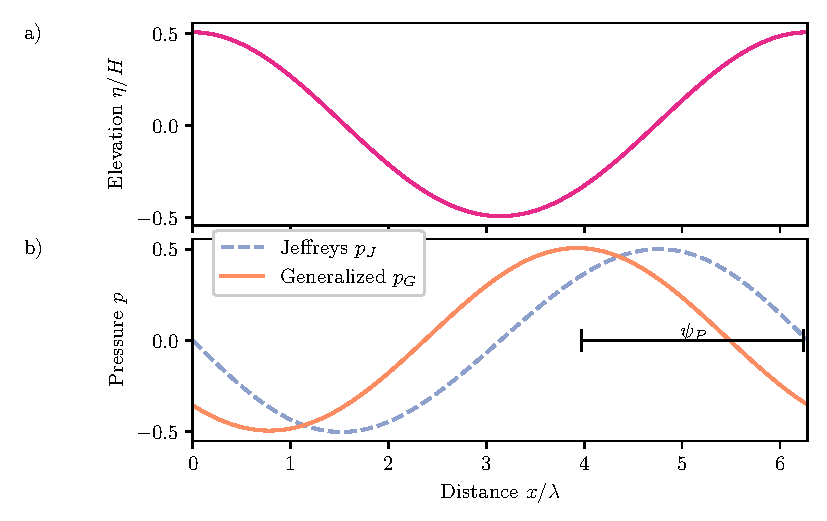
\includegraphics{Forcing-Types.eps}
  \caption{
    Forcing types with normalized nondimensional pressure P as a
    function of nondimensional distance $x/\lambda$.
  }
\end{figure}

\subsection{Jeffreys Forcing}
\begin{figure}
  \centering
  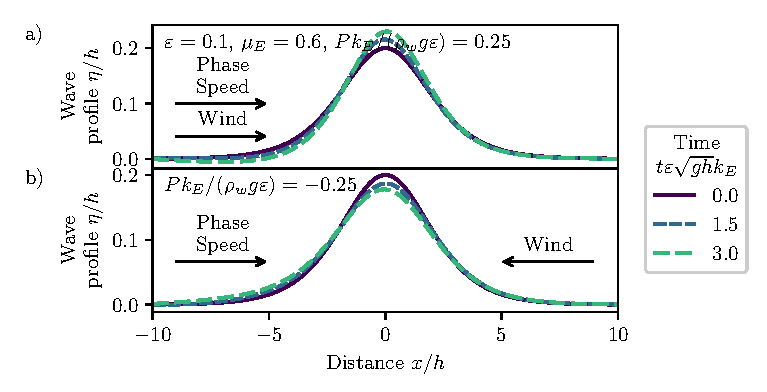
\includegraphics{Snapshots-Positive-Negative.eps}
  \caption{
    Evolution of a solitary wave profile under onshore and offshore Jeffreys
    forcing.
  }
\end{figure}

\begin{figure}
  \centering
  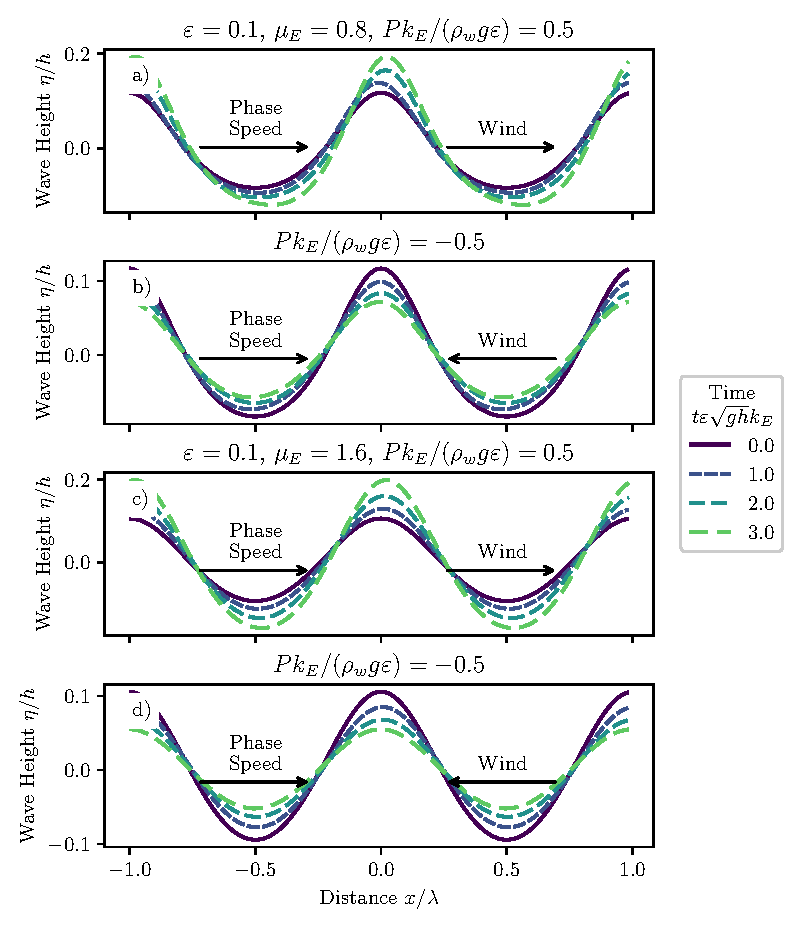
\includegraphics{Snapshots-Positive-Negative-Cnoidal.eps}
  \caption{
    Evolution of a cnoidal profile under onshore and offshore Jeffreys
    forcing.
  }
\end{figure}

\begin{figure}
  \centering
  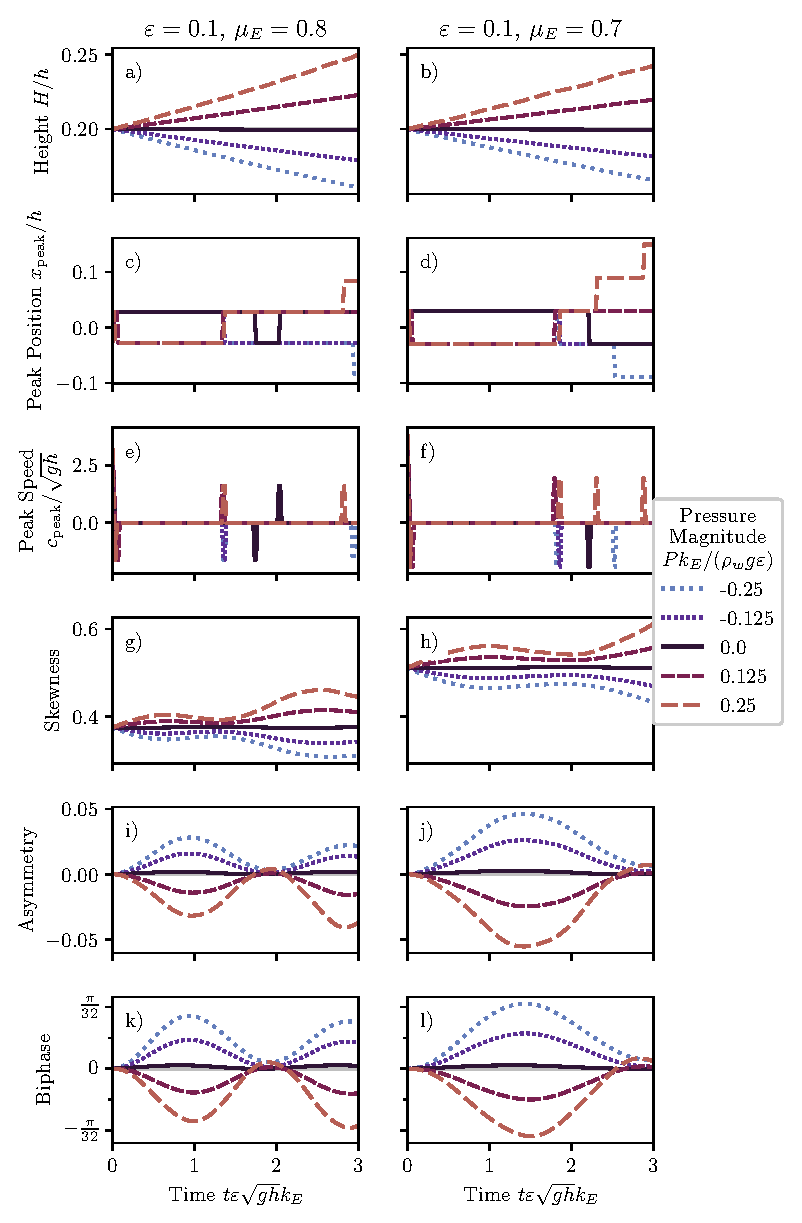
\includegraphics{Skew-Asymm-Cnoidal.eps}
  \caption{
    Skewness and asymmetry of cnoidal profile under onshore and offshore
    Jeffreys forcing.
  }
\end{figure}

\begin{figure}
  \centering
  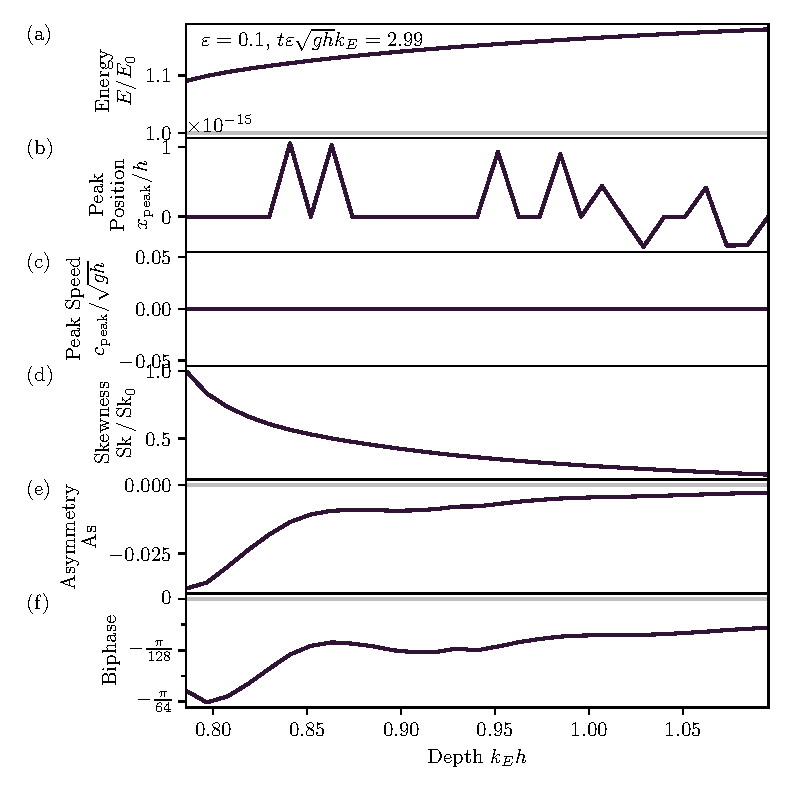
\includegraphics{Skew-Asymm-Cnoidal-kh.eps}
  \caption{
    Skewness and asymmetry of cnoidal profile under onshore forcing as a
    function of nondimensional depth $kh$.
  }
\end{figure}

\subsection{Generalized Miles Forcing}

\begin{figure}
  \centering
  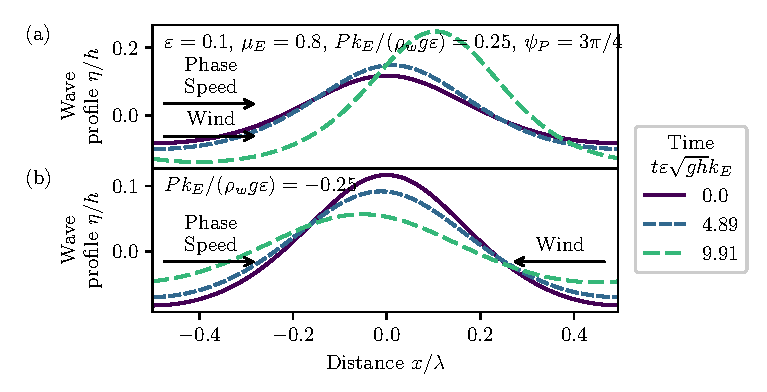
\includegraphics{Snapshots-Positive-Negative-Cnoidal-GM.eps}
  \caption{
    Evolution of a cnoidal profile under onshore and offshore Generalized
    Miles forcing.
  }
\end{figure}

\begin{figure}
  \centering
  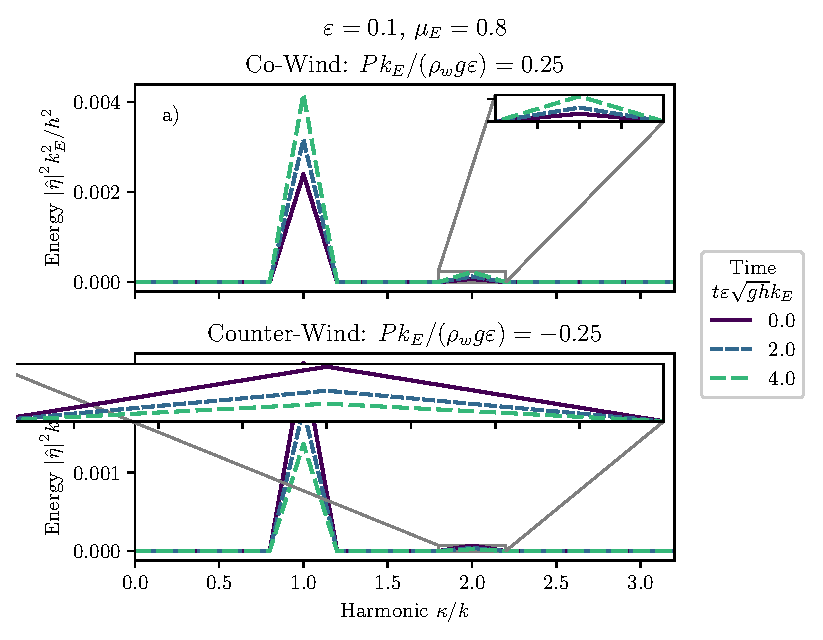
\includegraphics{Power-Spectrum-Jeffreys.eps}
  \caption{
    Power spectrum of cnoidal wave under Jeffreys forcing.
  }
\end{figure}

\begin{figure}
  \centering
  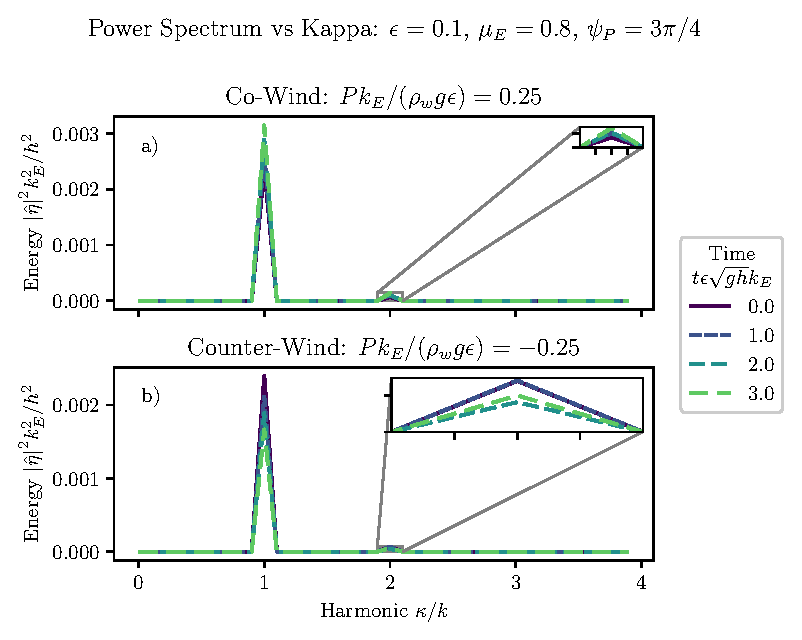
\includegraphics{Power-Spectrum-GM.eps}
  \caption{
    Power spectrum of cnoidal wave under Generalized Miles forcing.
  }
\end{figure}

\begin{figure}
  \centering
  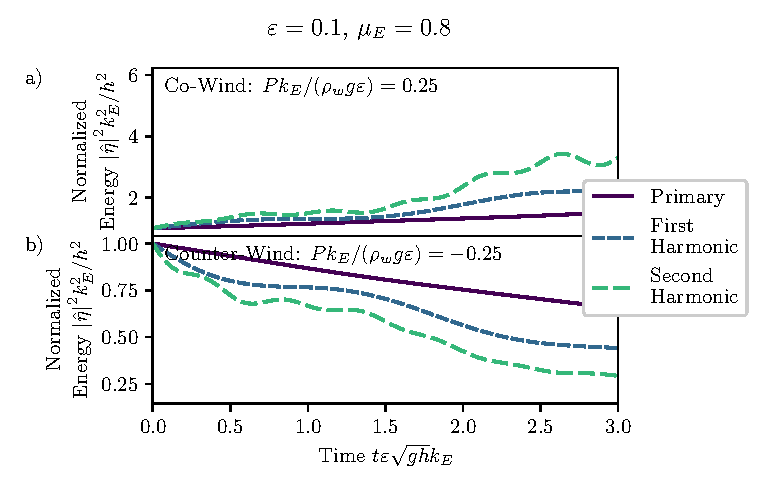
\includegraphics{Power-Spectrum-vs-Time-Jeffreys.eps}
  \caption{
    Power spectrum of cnoidal wave under Jeffreys forcing as a function
    of time.
  }
\end{figure}

\begin{figure}
  \centering
  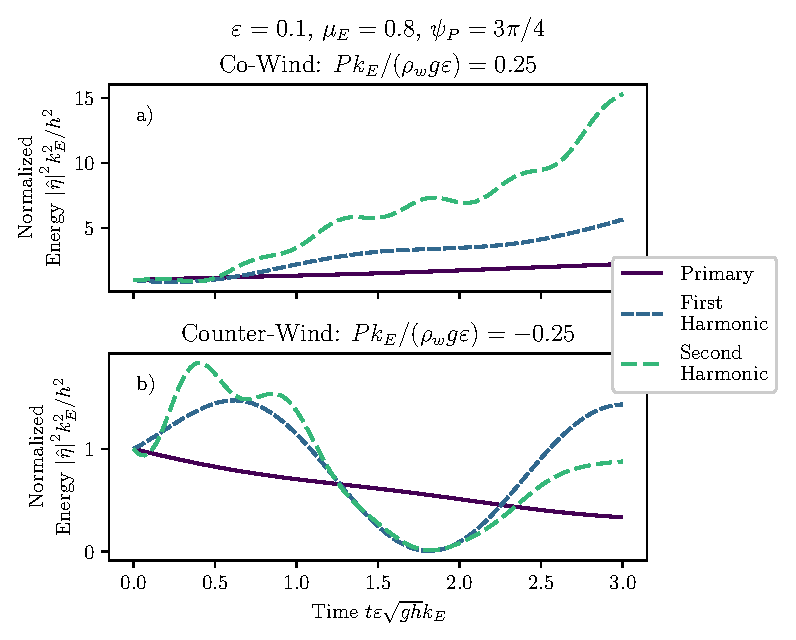
\includegraphics{Power-Spectrum-vs-Time-GM.eps}
  \caption{
    Power spectrum of cnoidal wave under Generalized Miles forcing as a
    function of time.
  }
\end{figure}

Note that the Generalized Miles type forcing seems inappropriate.
It appears to preferentially enhance the higher harmonics, which can be
seen by looking at the power spectrum $\abs{\hat{\eta}}^2$ as a function
of time.
In particular, when the wind is blowing \emph{against} the wave, the
second harmonic is \emph{enhanced}, whereas we expect all harmonics to
be suppressed.
Also, this seems to be more pronounced for large $\psi_P$, like $\psi_P
= 3\pi/4$, whereas small $\psi_P \ll 1$ show the expected behaviour.
This leads to the growth of the second harmonic large relative to the
primary, essentially bifurcating the crest.
Therefore, the Generalized Miles type forcing seems unrealistic.

This is not surprising.
If we temporarily include the pressure at leading order for simplicity,
the leading order equations become
\begin{gather}
  \pdv{\eta_0}{t_0} + \pdv[2]{\varphi_0}{x} = 0 \,, \\
  \eta_0 + \pdv{\varphi_0}{t_0} = -p_0 \,.
\end{gather}
Eliminating $\phi_0$ from this gives
\begin{equation}
  \pqty{\pdv[2]{t_0} - \pdv[2]{x} } \eta_0 = \pdv[2]{x} p_0 \,.
\end{equation}
Fourier transforming from $x$ to $m$ gives
\begin{equation}
  \pqty{\pdv[2]{t_0} + m^2 } \hat{\eta}_{0,m} = -m^2 \GenP
  \hat{\eta}_{0,m} \,.
\end{equation}
This gives
\begin{equation}
  \eta_0 \propto e^{\im(m x - \omega_m t_0)}
\end{equation}
with
\begin{equation}
  \omega_m = mk \sqrt{gh \pqty{1 + k \GenP}}
\end{equation}
where we have redimensionalized.
Then, the imaginary part of $\omega_m$ is
\begin{equation}
  \Im{\omega_m} = mk \sgn \pqty{\Im{\GenP}} \sqrt{\frac{gh}{2}} \sqrt{-1
    - k\Re{\GenP} + \sqrt{1 + k^2 \abs{\GenP}^2 + 2 k \Re{\GenP}}} \,.
\end{equation}
Crucially, notice that $\sgn[\Im{\omega_m}] = \sgn{\Im{\GenP}}$.
Therefore, if $\Im{\GenP}>0$, mode-$m$ grows; if $\Im{\GenP} <
0$, mode-$m$ shrinks.

First, consider the Jeffreys case, where $\GenP = \pm \im m P$.
For the co-wind case, the $(+)$ sign is chosen and $\Im{\GenP} > 0$ for
all modes, causing each harmonic to grow.
For the counter-wind case, the $(-)$ sign is chosen and $\Im{\GenP} < 0$
for all modes, causing each harmonic to shrink.
This is the expected behavior.

Consider now Generalized Miles, where $\GenP = P \exp(\im m \psi_P)$.
The plots are made for $\psi_P = \pm 3\pi/4$ (positive for
co-wind, negative for counter-wind).
For the co-wind case, $\Im{\POne} = P \cos(3\pi/4) > 0$ and the primary
grows, while $\Im{\PTwo} = P \cos(3\pi/2) = -P$ and the first harmonic
shrinks quickly.
Technically, the $m=6$ mode grows quicker than the primary (since
$\Im{\hat{P}_6} = P \cos(9\pi/2) = P$), but since it is so much smaller
than the primary, it takes a long time to become noticeable.

However, for the counter-wind case $\Im{\POne} = P \cos(-3\pi/4) < 0$ and the primary
shrinks, while $\Im{\PTwo} = P \cos(-3\pi/2) = P$ and the first harmonic
\emph{grows} quickly.
Thus, within a relatively short time, the first harmonic becomes
dominant.
Thus, GM is a poor choice.

For the Jeffreys case, we get the KdV-Burgers equation.
We can solve this numerically, though we will need an initial condition.
We will choose the solutions of the ordinary KdV equation as our initial
condition: cnoidal or solitary waves (which are a special case of
cnoidal waves).

In the general KdV case, we have
\begin{equation}
  \mathcal{A} \pdv{\eta_0}{t_1} + \mathcal{F} \pdv{\eta_0}{x} + \mathcal{B}
  \eta_0 \pdv{\eta_0}{x} + \mathcal{C} \pdv[3]{\eta_0}{x} = 0 \,.
\end{equation}
Using the solution in from \citet{dingemans1997water} (as quoted in
\citeauthor{brun2018convective}) and rescaling variables, the cnoidal
wave solution is
\begin{equation}
  \eta_0 = \eta_2 + H \cn^2\pqty{\frac{x-c_1 t}{\Delta} , m} \,,
  \label{eq:cnoidal_sol_nondim}
\end{equation}
with
\begin{gather}
  \eta_2 = \frac{H}{m} \pqty{1 - m - \frac{E(m)}{K(m)}}
  \qq{and}
  \Delta = \sqrt{\frac{12 \mathcal{C}}{\mathcal{B}} \frac{m}{H}}
  \label{eq:nondim_cnoidal_params}
  \\
  \qq{and}
  c_1 = \frac{\mathcal{F}}{\mathcal{A}} + \frac{2}{3} \frac{H}{m}
  \frac{\mathcal{B}}{\mathcal{A}} \pqty{1 - \frac{1}{2} m - \frac{3}{2}
    \frac{E(m)}{K(m)}} \,.
\end{gather}
Note that the (nondimensional) wavelength $\lambda$ is
\begin{equation}
  \lambda = 2 K(m) \Delta = K(m) \sqrt{\frac{48
  \mathcal{C}}{\mathcal{B}} \frac{m}{H}} \,.
  \label{eq:nondim_lambda}
\end{equation}
Here, $\cn$ is one of the Jacobi elliptic functions, and $K(m)$ and
$E(m)$ are the complete elliptic integrals of the first and second kind,
respectively, with $m \in [0,1]$ the elliptic parameter.

The solitary wave solution is
\begin{equation}
  \eta_0 = H \sech^2\pqty{\frac{x - c_1 t_1}{\Delta}} \,,
\end{equation}
with
\begin{equation}
  \Delta = \sqrt{\frac{12 \mathcal{C}}{\mathcal{B}} \frac{1}{H}}
  \qq{and}
  c_1 = \frac{\mathcal{F}}{\mathcal{A}} + \frac{H \mathcal{B}}{3
    \mathcal{A}} \,.
\end{equation}
Note that the solitary wave is recovered from the cnoidal wave as $m \to
1$ (note $E(m)/K(m) \to 0$ as $m \to 1$), and the linear wave
approximation is recovered as $m \to 0$.
Here, $\abs{H}$ is an order-1 parameter and $\sgn(H) = \sgn(\mathcal{B}
\mathcal{C})$.
For our particular system, we have $\mathcal{A} = 1$, $\mathcal{B} =
3/2$, $\mathcal{C} = \mu/(6\epsilon)$, and $\mathcal{F} = 0$.

\subsection{\label{sec:redim} Redimensionalization}
We can now redimensionalize; for clarity, we temporarily revert back to
dimensional variables (with primes denoting dimensionless).
It is important to recall that the various new parameters we have
defined ($\mathcal{A}$, $\mathcal{B}$, $\Delta$, $H$, \etc) are all
dimensionless and order unity.
We have some freedom in choosing how to redimensionalized these (if we
choose to at all).
The KdVB coefficients will be left as-is: since they only appear as
parameters with no intrinsic meaning, it would only clutter the formulas
if we redimensionalize.
However, the other new parameters ($\Delta$, $H$, $c_1$, \etc) should be
redimensionalized so that the resulting, dimensional equations and
definitions look similar the nondimensional equations.
For instance, if we were interested in plotting the Fourier transform of
$\eta$ as a function of $\kappa$ (conjugate to $x$), we would like the
Fourier transform in nondimensional form,
\[
  \hat{\eta'}(\kappa') = \int e^{\im \kappa' x'} \eta'(x') \dd{x'}
\]
to have the same form when expressed in dimensional quantities,
\[
  \hat{\eta'}(\kappa') = \int e^{\im \kappa' x k_E} \frac{\eta(x)}{a}
  \dd{x} k_E
  \implies \hat{\eta}(\kappa) = \int e^{\im \kappa x} \eta(x) \dd{x}
\]
giving the redimensionalizations  $\kappa \coloneqq \kappa' k_E$ and
$\hat{\eta} = \hat{\eta'} a/k_E$.
This resolves the ambiguity of redimensionalizing new parameters.

Now, beginning with our solution \cref{eq:cnoidal_sol_nondim}, we
redimensionalize as
\begin{equation}
  \begin{split}
  \frac{\eta_0}{\epsilon h} &= \eta_2' + H' \cn^2\pqty{\frac{k_E x - k_E
    \sqrt{gh} c_1' \epsilon t}{\Delta'}, m}
  \\
  \implies
  \eta_0 &= \epsilon h \eta_2' + \epsilon h H'
  \cn^2\pqty{\frac{k_E}{\Delta'} \bqty{x - \epsilon \sqrt{gh} c_1' t}, m}
  \\
  &\coloneqq \eta_2 + H \cn^2\pqty{\frac{x - c_1 t}{\Delta}, m} \,.
  \end{split}
\end{equation}
Here, we have defined the dimensional quantities $H$, $\eta_2$,
$\Delta$, and $c_1$:
\begin{gather}
  H = \epsilon h H'
  \qq{and}
  \eta_2 = \epsilon h \eta_2' = \frac{H}{m} \pqty{1 - m - \frac{E(m)}{K(m)}}
  \qq{and}
  \Delta = \frac{\Delta'}{k_E}
  \\
  \qq{and}
  c_1 = \epsilon \sqrt{gh} c_1' = \epsilon \sqrt{gh} \pqty{
    \frac{\mathcal{F}}{\mathcal{A}} + \frac{2}{3} \frac{H}{m}
    \frac{\mathcal{B}}{\mathcal{A}} \pqty{1 - \frac{1}{2} m - \frac{3}{2}
    \frac{E(m)}{K(m)}} }
\end{gather}
Given the conventional definition that $H = 2 a$, we have
\begin{equation}
  2 a = \epsilon h H' = a H' \implies H' = 2 \,.
\end{equation}
As $m \to 0$, we have $\cn \to \cos$, $K(m) \to \pi/2$ and $E(m) \to
\pi/2$, and we keep $H/m$ fixed.
This gives
\begin{equation}
  \eta_0 \to H \cos^2 \pqty{\frac{x-c_1 t}{\Delta}}^2
  = \frac{H}{2} \cos \pqty{\frac{2}{\Delta} \bqty{x-c_1 t}}
  \qq{as} m \to 0 \,.
\end{equation}
Since we want this to reduce to the usual $(H/2) \cos(k[x-c_1 t])$, we
define (for all $m$)
\begin{equation}
  k_E \coloneqq \frac{2}{\Delta}
\end{equation}
Note that \cref{eq:nondim_lambda} also means
\begin{equation}
  \lambda' = 2 K(m) \Delta' = 2 K(m) \Delta k_E = 4 K(m) \,.
\end{equation}
Note that, in particular, this means
\begin{equation}
  k = \frac{2 \pi}{\lambda} = \frac{2 \pi}{\lambda'} k_E
  = \frac{\pi}{2 K(m)} k_E \,.
\end{equation}
So, as $m \to 0$, $k \to k_E$, while $m \to 1$ yields $k \to 0$.

Finally, we can now fix $m$ as a function of $\mu$ and $\epsilon$:
\begin{equation}
  k_E = \frac{2}{\Delta} = \frac{2 k_E}{\Delta'}
  \implies \Delta' = 2 \,.
\end{equation}
However, using \cref{eq:nondim_cnoidal_params}, we have
\begin{equation}
  2 = \Delta ' = \sqrt{\frac{12 \mathcal{C}}{\mathcal{B}}
    \frac{m}{H'}}
  = \sqrt{\frac{12 \mathcal{C}}{\mathcal{B}} \frac{m}{2}}
  \implies m = \frac{2 \mathcal{B}}{3 \mathcal{C}} \,.
\end{equation}
For our particular values of $\mathcal{B} = 3/2$ and $\mathcal{C} =
\mu/(6 \epsilon)$, we have
\begin{equation}
  m = 6 \frac{\epsilon}{\mu} \,.
\end{equation}
Since $m \in [0,1]$, this implies $0 \le \epsilon \le \mu/6$.
Finally, note that since $m = 1$ gives the solitary wave solution, this
means that we have the requirement that
\begin{equation}
  \mu = 6 \epsilon
\end{equation}
for solitary waves; this is simply the well-known fact that the height
and width of a solitary wave satisfy a fixed relationship.

Therefore, the nondimensional equation we are solving is
\begin{equation}
  \mathcal{A} \pdv{\eta'_0}{t'_1} + \mathcal{F} \pdv{\eta'_0}{x'} + \mathcal{B}
  \eta'_0 \pdv{\eta'_0}{x'} + \mathcal{C} \pdv[3]{\eta'_0}{{x'}} = 0 \,.
\end{equation}
with $\mathcal{A} = 1$, $\mathcal{B} = 3/2$, $\mathcal{C} =
\mu/(6\epsilon)$, and $\mathcal{F} = 0$.
For our initial condition, we use
\begin{equation}
  \eta'_0(x) = \eta'_2 + 2 \cn^2\pqty{\frac{x'}{2} , m} \,,
\end{equation}
with
\begin{equation}
  \eta'_2 = \frac{2}{m} \pqty{1 - m - \frac{E(m)}{K(m)}}
\end{equation}

\section{\texorpdfstring{Weak Wind: $\alpha = \epsilon^{1.5}$}{Weak
Wind} \label{sec:weak}}
Here, we assume $\alpha \coloneqq P k/(\rho_w g) = \epsilon^{1.5}$.
Technically, we should expand our functions $\eta$, $\varphi$, and $p$,
as well as our timescales $t_n$ in powers of $\epsilon^{0.5}$ now.
That is, we now write
\begin{equation}
  \eta(x,t) = \eta_0(x,t_0,t_{0.5},t_1,\ldots) + \epsilon^{0.5}
  \eta_{0.5}(x,t_0,t_{0.5},t_1,\ldots) + \epsilon
  \eta_1(x,t_0,t_{0.5},t_1,\ldots) + \ldots \,,
\end{equation}
with similar expansions for $\varphi$ and $p$.
Now, time derivatives become
\begin{equation}
  \pdv{t} = \pdv{t_0} + \epsilon^{0.5} \pdv{t_{0.5}} + \epsilon
  \pdv{t_1} + \ldots \,.
\end{equation}

\subsection{Zeroth Order Equations}
The order-one $\order{\epsilon^0}$ equations and solutions are unchanged
from \cref{sec:intermediate}:
\begin{align}
  \varphi_0 &= f_0(x-t_0,t_{0.5},t_1) + g_0(x+t_0,t_{0.5},t_1) \,, \\
  \eta_0 &= - \pdv{\varphi_0}{t_0} = f_0'(x-t_0,t_{0.5},t_1) -
    g_0'(x+t_0,t_{0.5},t_1) \,,
\end{align}
Again, we restrict to right-moving waves by taking $g_0=0$.

\subsection{Order \texorpdfstring{$\epsilon^{0.5}$}{0.5} Equations}
Going to the next order, $\order{\epsilon^{0.5}}$, we have
\begin{gather}
  \pdv{\eta_{0.5}}{t_0} + \pdv[2]{\varphi_{0.5}}{x} =
  -\pdv{\eta_0}{t_{0.5}} \,, \\
  \eta_{0.5} + \pdv{\varphi_{0.5}}{t_0} = -\pdv{\varphi_0}{t_{0.5}}\,.
\end{gather}
If we take $\pdv*{\eta_0}{t_{0.5}} = \pdv*{\varphi_0}{t_{0.5}} = 0$,
this reduces to the homogeneous, zeroth order equations,
\cref{eq:zero_order_kin,eq:zero_order_dyn}.
Since we will be going to a higher order, we need to ensure the
asymptotic expansion remains ordered, with $\eta_0 \gg \epsilon^{0.5}
\eta_{0.5}$~\citep{ott1969nonlinear}; therefore, it is useful to
retain $\eta_{0.5} \neq 0$.
Thus, we find that $\eta_{0.5}$ and $\varphi_{0.5}$ are also travelling
waves:
\begin{align}
  \varphi_{0.5} &= f_{0.5}(x-t_0,t_{0.5},\ldots) \,,
    \label{eq:phi0.5_sol} \\
  \eta_{0.5} &= f_{0.5}'(x-t_0,t_{0.5},\ldots) \,.
    \label{eq:eta0.5_sol}
\end{align}

\subsection{First Order Equations}
Continuing to the next order of perturbation theory, we retain terms of
order $\order{\epsilon}$.
Inserting our previous solutions,
\cref{eq:phi0_sol,eq:eta0_sol,eq:phi0.5_sol,eq:eta0.5_sol} yields
\begin{gather}
  \begin{aligned}
    \pdv{\eta_1}{t_0} + \pdv[2]{\varphi_{1}}{x} &=
      -\pdv{\eta_{0.5}}{t_{0.5}}
      -\pdv{\eta_0}{t_1} - \pdv{x} \pqty{\eta_0 \pdv{\varphi_0}{x}} +
      \frac{1}{6} \pdv[4]{\varphi_0}{x} \\
    &= -\pdv{f_{0.5}'}{t_{0.5}} -\pdv{f_0'}{t_1} - 2 f_0' f_0'' +
      \frac{1}{6} f_0^{(4)} \,,
  \end{aligned}
  \\
  \begin{aligned}
    \eta_1 + \pdv{\varphi_1}{t_0} &= -\pdv{\varphi_0}{t_1}
      - \pdv{\varphi_{0.5}}{t_{0.5}}
      + \frac{1}{2} \frac{\partial^3 \varphi_0}
        {\partial t_0 \partial^2 x}
      - \frac{1}{2} \pqty{ \pdv{\varphi_0}{x} }^2 \\
    &= -\pdv{f_{0.5}}{t_{0.5}} -\pdv{f_0}{t_1} - \frac{1}{2} f_0^{(3)} -
      \frac{1}{2} \pqty{f_0'}^2 \,.
  \end{aligned}
\end{gather}

We are free to choose $\pdv*{t_{0.5}}{f_{0.5}} = 0$ (ensuring that $f_0$
and $f_{0.5}$ have the same $t_{0.5}$ dependence).
Then, these are the same equations as in \cref{sec:int_first_order} upon
taking $p_0=0$.
Therefore, repeating the same steps as before, we choose
\cref{eq:phi1_sol,eq:eta1_sol}
\begin{align}
  \varphi_1 = f_1(x-t_0,t_{0.5},\ldots) \,, \\
  \eta_1 = f_1'(x-t_0,t_{0.5},\ldots) \,.
\end{align}
and arrive at \cref{eq:kdv_burgers}, though with $P_J =0$ it reduces to
the KdV equation:
\begin{equation}
  \pdv{\eta_0}{t_1} + \frac{3}{2} \eta_0 \eta_0' + \frac{1}{6}
    \eta_0^{(3)} = 0 \,.
\end{equation}

\subsubsection{Solution to KdV Equation}
Now, we seek travelling wave solutions of the form
\begin{equation}
  \eta_0(x-t_0,t_1,t_{1.5}) = h_0(x-t_0-c_1 t_1,t_{1.5}) \,,
\end{equation}
with $c_1 \in \mathbb{R}$.
This gives
\begin{equation}
  \mathcal{L}_0[h_0] \coloneqq
    -c_1 h_0' + \frac{3}{2} h_0 h_0' + \frac{1}{6} h_0^{(3)} = 0 \,,
  \label{eq:L0_kernel}
\end{equation}
with $h_0' \coloneqq \eval{\pdv*{\theta}
h_0(\theta,t_{1.5})})_{\theta=x-t_0-c_1 t_1}$.
Here we have defined the linear operator $\mathcal{L}_0$
\begin{equation}
  \mathcal{L}_0 \coloneqq -c_1 \pdv{\theta} + \frac{3}{2} h_0
    \pdv{\theta} + \frac{1}{6} \pdv[3]{\theta} \,,
  \label{eq:L0_def}
\end{equation}
with $\theta \coloneqq x - t_0 - c_1 t_1$.
Integrating once yields
as $x \to \pm \infty$ yields
\begin{equation}
   -c_1 h_0 + \frac{3}{4} h_0^2 + \frac{1}{6} h_0'' = B_1 \,.
\end{equation}
Multiplying by $h_0'$ and integrating again gives
\begin{equation}
  -c_1 h_0^2 + \frac{1}{4} h_0^3 + \frac{1}{12} \pqty{h_0'}^2 = B_1 h_0
    + B_2 \,,
\end{equation}
which implies
\begin{equation}
  \frac{1}{3} \pqty{h_0'}^2 = - h_0^3 + 4 c_1 h_0^2 + B_1 h_0 + B_2
    = \pqty{H_1 - h_0} \pqty{H_2 - h_0} \pqty{H_3 - h_0}
\end{equation}
where we have redefined $4 B_1 \to B_1$ and $4 B_2 \to B_2$ and defined
$H_1 < H_2 < H_3$.
This can be solved in terms of the Jacobi elliptic
functions~\citep[\eg][]{mei2005nonlinear}:
\begin{equation}
  \eta_0 = H_2 + (H_3 - H_2) \cn^2\bqty{\frac{\sqrt{3}}{2} \sqrt{H_3 -
    H_1} \pqty{x - t_0 - c_1 t_1}} \,.
  \label{eq:eta0_cn}
\end{equation}
\textbf{TODO: express $H_1$, $H_2$, and $H_3$ in terms of $B_1$, $B_2$,
and $c_1$.}

\subsection{Order \texorpdfstring{$\epsilon^{1.5}$}{1.5} Equations}
Now, retaining $\order{\epsilon^{1.5}}$ terms, we finally have the
introduction of a pressure forcing $p_0$:
\begin{gather}
  \begin{aligned}
    \pdv{\eta_{1.5}}{t_0} + \pdv[2]{\varphi_{1.5}}{x} &=
      -\pdv{\eta_{1}}{t_{0.5}}
      -\pdv{\eta_{0.5}}{t_{1}}
      -\pdv{\eta_{0}}{t_{1.5}}
      - \pdv{x} \pqty{\eta_{0.5} \pdv{\varphi_0}{x} + \eta_0
      \pdv{\varphi_{0.5}}{x}} + \frac{1}{6} \pdv[4]{\varphi_0.5}{x} \\
    &= -\pdv{f_1'}{t_{0.5}} -\pdv{f_0'}{t_{1.5}} -\pdv{f_{0.5}'}{t_1}
      -2 f_{0.5}' f_0'' -2 f_0' f_{0.5}'' + \frac{1}{6} f_{0.5}^{(4)}
      \,,
  \end{aligned}
  \\
  \begin{aligned}
    \eta_{1.5} + \pdv{\varphi_{1.5}}{t_0} &=
      -p_0
      -\pdv{\varphi_1}{t_{0.5}}
      -\pdv{\varphi_{0.5}}{t_1}
      -\pdv{\varphi_0}{t_{1.5}}
      - \pdv{\varphi_{0.5}}{t_{0.5}}
      + \frac{1}{2} \frac{\partial^3 \varphi_{0.5}}
        {\partial t_0 \partial^2 x}
      - \pdv{\varphi_0}{x} \pdv{\varphi_{0.5}}{x} \\
    &= -p_0
      -\pdv{f_1}{t_{0.5}}
      -\pdv{f_{0.5}}{t_1}
      -\pdv{h_0}{t_{1.5}}
      - \frac{1}{2} f_{0.5}^{(3)} - h_0' f_{0.5}' \,.
  \end{aligned}
\end{gather}
Then, combining the equations to eliminate $\eta_{1.5}$ yields
\begin{equation}
  \pqty{\pdv[2]{x} - \pdv[2]{t_0}} \varphi_{1.5} =
    -2 \pdv{f_1'}{t_{0.5}}
    -2 \pdv{f_{0.5}'}{t_1}
    -2 \pdv{h_0'}{t_{1.5}}
    + \pdv{p_0}{t_0}
    - 3 h_0' f_{0.5}''
    - 3 f_{0.5}' h_0''
    - \frac{1}{3} f_{0.5}^{(4)}
    \,.
\end{equation}

We begin by choosing
\begin{align}
  \varphi_{1.5} = f_{1.5}(x-t_0,t_{0.5},\ldots) \,, \\
  \eta_{1.5} = f_{1.5}'(x-t_0,t_{0.5},\ldots) \,,
\end{align}
so that $\eta_{1.5}$ has the same $t_0$ dependence as $\eta_0$.
Additionally, we impose $\pdv*{f_1}{t_{0.5}} = 0$ so that it has the
same $t_{0.5}$ dependence as $f_0$.
Thus, we find
\begin{equation}
  \pdv{f_{0.5}'}{t_1}
    + \frac{3}{2} h_0' f_{0.5}''
    + \frac{3}{2} f_{0.5}' h_0''
    - \frac{1}{6} f_{0.5}^{(4)}
  =
  - \pdv{f_0'}{t_{1.5}}
    + \frac{1}{2} \pdv{p_0}{t_0}
    \,.
\end{equation}
Additionally, we assume $\eta_{0.5}$ has the same $t_1$ dependence as
$\eta_0$:
\begin{equation}
  \eta_{0.5}(x-t_0,t_1,t_{1.5},\ldots) = h_{0.5}(x - t_0 - c_1 t_1,
    t_{1.5}, \ldots) \,.
\end{equation}
Then, we finally obtain
\begin{equation}
  \mathcal{L}_{0.5} [h_{0.5}] \coloneqq
    -c_1 h_{0.5}'
    + \frac{3}{2} h_0 h_{0.5}'
    + \frac{3}{2} h_{0.5} h_0'
    - \frac{1}{6} h_{0.5}^{(3)}
  =
  - \pdv{h_0}{t_{1.5}}
    + \frac{1}{2} \pdv{p_0}{t_0}
    \,,
  \label{eq:L0.5_def}
\end{equation}
where we have defined the linear operator $\mathcal{L}_{0.5}$

Now, the right-hand side must be orthogonal to all functions $F$ in the
kernel of $\mathcal{L}_{0.5}^{\dagger}$, \ie the adjoint of
$\mathcal{L}_{0.5}$.
To see this, we can simply multiply both sides by a function $F(\theta)$
such that $\mathcal{L}_{0.5}^{\dagger}[F] = 0$ and integrate over
$\theta = x-t_0-c_1 t_1$:
\begin{equation}
  \int F \mathcal{L}_{0.5} [\eta_{0.5}] \dd{\theta}
  = \int \eta_{0.5} \mathcal{L}_{0.5}^{\dagger} [F] \dd{\theta}
  = 0
  =
  \int \pqty{- \pdv{h_0}{t_{1.5}} + \frac{1}{2} \pdv{p_0}{t_0}}
    F \dd{\theta} \,,
\end{equation}
where the first equality follows from the definition of an adjoint
operator, and the second follows from the definition of $F$ being in the
kernel of $\mathcal{L}_{0.5}^{\dagger}$.
The last equation is the definition of two functions ($F$ and the
right-hand side of \cref{eq:L0.5_def}) being orthogonal.

However, we already know the adjoint of $\mathcal{L}_{0.5}$; it is easy
to show that $\mathcal{L}_{0.5}^{\dagger} = -\mathcal{L}_0$, defined in
\cref{eq:L0_def}.
In particular, this means
\begin{equation}
  \int \dd{\theta} n_0 \mathcal{L}_{0.5} [n_{0.5}]
  = -\int \dd{\theta} n_{0.5} \mathcal{L}_{0.5} [n_0]
  \implies
  0 = \int \dd{\theta} \pqty{n_0 \mathcal{L}_{0.5} [n_{0.5}] + n_{0.5}
    \mathcal{L}_{0.5} [n_0] } \,.
\end{equation}
However, as shown in \cref{eq:L0_kernel}, our solutions $\eta_0 = h_0$
already span the kernel of $\mathcal{L}_0 =
-\mathcal{L}_{0.5}^{\dagger}$.
Therefore, our compatibility condition is
\begin{equation}
  0 = \int \pqty{- \pdv{h_0}{t_{1.5}} + \frac{1}{2} \pdv{p_0}{t_0}}
    h_0(\theta) \dd{\theta} \,.
\end{equation}

Now, we insert our solution \cref{eq:eta0_cn}
\begin{equation}
  h_0(\theta) = H_2 + (H_3 - H_2) \cn^2\bqty{\frac{\sqrt{3}}{2} \sqrt{H_3 -
    H_1} \theta } \,.
\end{equation}
while recalling that $H_1$, $H_2$, and $H_3$, and $c_1$ in $\theta = x -
t_0 - c_1 t_1$ (only three of which are linearly independent) may depend
on $t_{1.5}$.
\textbf{TODO: finish calculation of $c_1(t_{1.5})$ dependence}

Finally, we can now use \cref{eq:L0.5_def} to calculate $h_{0.5}$.
\textbf{TODO: finish calculation of $h_{0.5}$}

\subsection{Order \texorpdfstring{$\epsilon^{2}$}{2} Equations}
Now, retaining $\order{\epsilon^2}$ terms, we find
\textbf{TODO: finish}

\section{\texorpdfstring{Strong Wind: $\alpha = 1$}{Strong Wind};
Discrete Sum}
Here, we assume $\alpha \coloneqq P k/(\rho_w g) = 1$.

\subsection{Zeroth Order Equations}
Collecting order-one terms $\order{\epsilon^0}$ from
\cref{eq:kinematic_bc_varphi,eq:dynamic_bc_varphi} gives
\begin{gather}
  \pdv{\eta_0}{t_0} + \pdv[2]{\varphi_0}{x} = 0 \,, \\
  p_0 + \eta_0 + \pdv{\varphi_0}{t_0} = 0 \,.
\end{gather}
Fourier transforming from $x$ to $m$ gives
\begin{gather}
  \pdv{\hat{\eta}_0}{t_0} - m^2  \hat{\varphi}_0 = 0 \,, \\
  \hat{p}_0 + \hat{\eta}_0 + \pdv{\hat{\varphi}_0}{t_0} = 0 \,.
\end{gather}
Using the fact that $\hat{p} = \GenP \hat{\eta}$ and eliminating
$\hat{\eta}$, we find
\begin{equation}
  \bqty{\pdv[2]{t_0} + m^2 \pqty{1+\GenP}} \hat{\varphi}_0 = 0 \,.
\end{equation}
This is the standard one-dimensional wave equation and has solutions
\begin{equation}
  \hat{\varphi}_0 = A_m e^{-\im \omega_{0,m} t_0} + B_m e^{\im
    \omega_{0,m} t_0} \,,
\end{equation}
with
\begin{equation}
  \omega_{0,m} = \pm m \sqrt{1 + \GenP} \,.
\end{equation}
Notice that, while the unforced case has a nondispersive phase speed
\[
  c_{m, P=0} = \frac{\omega_{0,m}}{m} = \pm 1 \,,
\]
the forced case is now dispersive (since $\GenP$ varies between Fourier
modes)
\[
  c_m = \frac{\omega_{0,m}}{m} = \pm \sqrt{1 + \GenP} \,.
\]
We will restrict to unidirectional waves by taking $B_m = 0$, and we
redefine $A_m$ to give
\begin{equation}
  \hat{\varphi}_0 = - A_0 x + C_0 t_0 + \sum_{m=1}^{\infty} \im
    \frac{\omega_{0,m}}{m^2} A_m e^{-\im \omega_{0,m} t_0}
  \qq{with} \omega_{0,m} = \pm \sqrt{1+\GenP} \,.
\end{equation}
Here, we factored out the $0$-mode for convenience.
We have assumed \cref{eq:celerity_definition} that $\overline{u} = 0$,
which implies $A_0 = 0$.
Additionally, we find
\begin{equation}
  \hat{\eta}_0 = - \frac{1}{1+\GenP} \pdv{\hat{\varphi}_0}{t_0} =
    C_0 +
    \sum_{m=1}^{\infty} A_m e^{-\im \omega_{0,m} t_0} \,.
\end{equation}
Here, we use the fact that our datum is at the MWL to set $C_0 = 0$.
Fourier transforming back to $x$-space yields
\begin{align}
  \eta_0 &= \Re \sum_{m=1}^{\infty} A_m
    e^{\im (m x-\omega_{0,m} t_0)} \,, \\
  \varphi_0 &= -\Re \sum_{m=1}^{\infty} \im \frac{\omega_{0,m}}{m^2} A_m
    e^{\im (m x-\omega_{0,m} t_0)} \,.
\end{align}

\subsection{First Order Equations}
Considering now terms of order $\order{\epsilon}$ and inserting the
$\order{\epsilon^0}$ solutions, \cref{eq:phi0_sol,eq:eta0_sol}, we find
\begin{gather}
  \begin{aligned}
    \pdv{\eta_1}{t_0} + \pdv[2]{\varphi_{1}}{x} &=
      -\pdv{\eta_0}{t_1} - \pdv{x} \pqty{\eta_0 \pdv{\varphi_0}{x}} +
      \frac{1}{6} \pdv[4]{\varphi_0}{x} \\
    &= -\Re \sum_{m=1}^{\infty} \pqty{ \pdv{A_m}{t_1} + \frac{m^2}{6}
      \im \omega_0 A_m
      + \frac{1}{2} A_m \sum_{q \in \mathbb{Z} \setminus \{0\}}
      \im \omega_{0,q} \frac{m+q}{q} A_q e^{\im q (x-\omega_{0,q} t_0)}
      } e^{\im (m x-\omega_{0,m} t_0)}
    \,,
  \end{aligned}
  \\
  \begin{aligned}
    p_1 + \eta_1 + \pdv{\varphi_1}{t_0} &= - \pdv{\varphi_0}{t_1}
      + \frac{1}{2} \frac{\partial^3 \varphi_0}{\partial t_0 \partial^2 x}
      - \frac{1}{2} \pqty{ \pdv{\varphi_0}{x} }^2 \\
    &= \Re \sum_{m=1}^{\infty} \pqty{\im \frac{\omega_0}{m^2}
      \pdv{A_m}{t_1} + \frac{1}{2} \omega_0^2 A_1
      -\frac{1}{2} A_m \frac{\omega_{0,m}}{m} \sum_{q \in \mathbb{Z}
      \setminus \{0\}} \frac{\omega_{0,q}}{\abs{q}} A_q e^{\im q (x -
      \omega_{0,q} t_0)}
      } e^{\im (m x-\omega_{0,m} t_0)}
    \,.
  \end{aligned}
\end{gather}
Taking a Fourier transform, we find
\begin{gather}
  \begin{aligned}
  \pdv{\hat{\eta}_{1,m}}{t_0} - m^2 \hat{\varphi}_{1,m}
  &= -\pqty{ \pdv{A_m}{t_1} + \frac{m^2}{6}
      \im \omega_{0,m} A_m
      } e^{-\im \omega_{0,m} t_0} \\
  &\qquad
      - \frac{1}{2} \sum_{q \in \mathbb{Z} \setminus \{0\}}
      \im \omega_{0,q} \frac{m}{q} A_{m-q}
      A_q e^{-\im \omega_{0,q} t_0} e^{-\im \omega_{0,m-q} t_0}
    \,,
  \end{aligned}
  \\
  \begin{aligned}
  \hat{p}_{1,m} + \hat{\eta}_{1,m} + \pdv{\hat{\varphi}_{1,m}}{t_0}
  &= \pqty{\im \frac{\omega_{0,m}}{m^2}
    \pdv{A_m}{t_1} + \frac{1}{2} \omega_{0,m}^2 A_m
      } e^{-\im \omega_{0,m} t_0} \\
  &\qquad
      -\frac{1}{2} \sum_{q \in \mathbb{Z} \setminus \{0\}}
      \frac{\omega_{0,m-q}}{m-q} \frac{\omega_{0,q}}{\abs{q}} A_{m-q}
      A_q e^{-\im \omega_{0,q} t_0}  e^{-\im \omega_{0,m-q} t_0}
    \,.
  \end{aligned}
\end{gather}

Inserting $\hat{p}_{1,m} = \GenP \hat{\eta}_{1,m}$ and eliminating
$\hat{\varphi}_{1,m}$ yields
\begin{gather}
  \begin{aligned}
    &\pdv[2]{\hat{\eta}_{1,m}}{t_0} + m^2 \pqty{1+\GenP} \hat{\eta}_{1,m}
      = \pqty{ 2 \im \omega_{0,m} \pdv{A_m}{t_1} + \frac{m^2}{3}
      \omega_{0,m}^2 A_m } e^{-\im \omega_{0,m} t_0} \\
    &\qquad
      + \frac{1}{2} \sum_{q \in \mathbb{Z} \setminus \{0\}}
      \pqty{ -\omega_{0,q} \frac{m}{q} (q \omega_{0,q} + (m-q)
        \omega_{0,m-q})
      + \frac{\omega_{0,m-q}}{m-q} \frac{\omega_{0,q}}{\abs{q}} m^2
      }
      A_{m-q} A_q e^{-\im \omega_{0,q} t_0}
      e^{-\im \omega_{0,m-q} t_0}
    \,.
  \end{aligned}
\end{gather}

\section{\texorpdfstring{Strong Wind: $\alpha = 1$}{Strong Wind}:
Integral}
Here, we assume $\alpha \coloneqq P k/(\rho_w g) = 1$.
The continuous Fourier transform from $x$ to $\kappa$
will be $\hat{f}(\kappa) = \int_{-\infty}^{\infty} \dd{x} f(x) \exp(\im \kappa
x)$.
Further, since we are using integrals now, we will need the continuous
Fourier transform of the pressure:
\[
  p(x,t) = f(x) \star \eta(x,t) \implies \hat{p}(\kappa) = k \GenPk
    \hat{\eta}(\kappa) \,,
\]
with $\GenPk$ are arbitrary function of $\kappa$ that is linear in the
magnitude of the pressure forcing, $P$.
In particular, it takes the values $\GenPk = (\kappa/k) P_J \exp(\im \psi_P)$ with
$\psi_P = \pm \thalf \pi$ for Jeffreys, $\GenPk = P_M \exp[\im
\psi_P \sgn(\kappa/k)]$ for Miles, and $\GenPk = P_G \exp(\im \psi_P
\kappa/k)$ for Generalized.

\subsection{Zeroth Order Equations}
Collecting order-one terms $\order{\epsilon^0}$ from
\cref{eq:kinematic_bc_varphi,eq:dynamic_bc_varphi} gives
\begin{gather}
  \pdv{\eta_0}{t_0} + \pdv[2]{\varphi_0}{x} = 0 \,, \\
  p_0 + \eta_0 + \pdv{\varphi_0}{t_0} = 0 \,.
\end{gather}
Taking the continuous Fourier transform from $x$ to $\kappa$
($\hat{f}(\kappa) = \int_{-\infty}^{\infty} \dd{x} f(x) \exp(\im \kappa
x)$) gives
\begin{gather}
  \pdv{\hat{\eta}_0}{t_0} - \kappa^2  \hat{\varphi}_0 = 0 \,, \\
  \hat{p}_0 + \hat{\eta}_0 + \pdv{\hat{\varphi}_0}{t_0} = 0 \,.
\end{gather}
Using the fact that $\hat{p} = \GenPk \hat{\eta}$ and eliminating
$\hat{\eta}$, we find
\begin{equation}
  \bqty{\pdv[2]{t_0} + \kappa^2 \pqty{1+\GenPk}} \hat{\varphi}_0 = 0 \,.
\end{equation}
This is the standard one-dimensional wave equation and has solutions
\begin{equation}
  \hat{\varphi}_0(\kappa,t_0,t_1) =
  \begin{cases}
    A(\kappa,t_1) e^{-\im \omega_{0,\kappa} t_0} + B(\kappa,t_1)
      e^{\im \omega_{0,\kappa} t_0} & \kappa \neq 0 \\
    C_0(t_1) t_0 & \kappa = 0
  \end{cases} \,,
\end{equation}
with
$A(-\kappa) = A^*(\kappa)$, $B(-\kappa) = B^*(\kappa)$, and
\begin{equation}
  \omega_{0,\kappa} = \pm \kappa \sqrt{1 + \GenPk} \,.
\end{equation}
Notice that, while the unforced case has a nondispersive phase speed
\[
  c_{\kappa, P=0} = \frac{\omega_{0,\kappa}}{\kappa} = \pm 1 \,,
\]
the forced case is now dispersive (since $\GenPk$ varies between Fourier
modes)
\[
  c_{\kappa} = \frac{\omega_{0,\kappa}}{\kappa} = \pm \sqrt{1 + \GenPk}
  \,.
\]
We will restrict to unidirectional waves by taking $B(\kappa) = 0$, and
we redefine $A(\kappa)$ to give
\begin{equation}
  \hat{\varphi}_0 = C_0 t_0 + \int_{\kappa \neq 0} \im
    \frac{1}{2} \frac{\omega_{0,\kappa}}{\kappa^2} A(\kappa) e^{-\im
    \omega_{0,\kappa} t_0} \dd{\kappa}
  \qq{with} \omega_{0,\kappa} = \pm \sqrt{1+\GenPk} \,.
\end{equation}
Additionally, we find
\begin{equation}
  \hat{\eta}_0 = - \frac{1}{1+\GenPk} \pdv{\hat{\varphi}_0}{t_0} =
    -\frac{C_0}{1+\GenPk} +
    \int_{\kappa \neq 0} \frac{1}{2} A(\kappa) e^{-\im \omega_{0,\kappa}
    t_0} \dd{\kappa}
    \,.
\end{equation}
Here, we use the fact that our datum is at the MWL to set $C_0 = 0$.
Fourier transforming back to $x$-space yields
\begin{align}
  \eta_0 &= \frac{1}{2} \int_{-\infty,\kappa \neq 0}^{\infty} A(\kappa)
    e^{\im (\kappa x-\omega_{0,\kappa} t_0)} \,, \label{eq:eta0_sol_int2}
    \\
  \varphi_0 &= -\frac{1}{2} \int_{-\infty,\kappa \neq 0}^{\infty} \im
    \frac{\omega_{0,\kappa}}{\kappa^2} A(\kappa)
    e^{\im (\kappa x-\omega_{0,\kappa} t_0)} \label{eq:phi0_sol_int2} \,,
\end{align}
with $A(-\kappa) = A^*(\kappa)$.

\subsection{First Order Equations}
Considering now terms of order $\order{\epsilon}$, we find
\begin{gather}
    \pdv{\eta_1}{t_0} + \pdv[2]{\varphi_{1}}{x} =
      -\pdv{\eta_0}{t_1} - \pdv{x} \pqty{\eta_0 \pdv{\varphi_0}{x}} +
      \frac{1}{6} \pdv[4]{\varphi_0}{x} \,, \\
    p_1 + \eta_1 + \pdv{\varphi_1}{t_0} = - \pdv{\varphi_0}{t_1}
      + \frac{1}{2} \frac{\partial^3 \varphi_0}{\partial t_0 \partial^2 x}
      - \frac{1}{2} \pqty{ \pdv{\varphi_0}{x} }^2     \,.
\end{gather}
Eliminating $\varphi_1$ gives
\begin{equation}
    \pdv[2]{x} \pqty{p_1 + \eta_1} - \pdv[2]{\eta_1}{t_0} =
      \pdv{t_1} \pqty{ \pdv{\eta_0}{t_0} - \pdv[2]{\varphi_0}{x} }
      + \frac{1}{3} \frac{\partial^5 \varphi_0}{\partial t_0 \partial^4
      x}
      + \pdv{x} \pqty{ -\pdv{\varphi_0}{x} \pdv[2]{\varphi_0}{x} +
      \pdv{\eta_0}{t_0} \pdv{\varphi_0}{x} + \eta_0
      \pdv{\varphi_0}{t_0}{x} } \,.
\end{equation}
Using $\pdv*[2]{\varphi_0}{x} = -\pdv*{\eta_0}{t_0}$, we find
\begin{equation}
  \pdv[2]{x} \pqty{p_1 + \eta_1} - \pdv[2]{\eta_1}{t_0} =
    2 \pdv{\eta_0}{t_1}{t_0}
    - \frac{1}{3} \frac{\partial^4 \eta_0}{\partial^2 t_0 \partial^2 x}
    + \pdv{x} \bqty{2 \pdv{\eta_0}{t_0} \pdv{\varphi_0}{x}
    + \eta_0 \pdv{\varphi_0}{t_0}{x}} \,.
\end{equation}
Taking an $x$-$\kappa$ Fourier transform gives
\begin{equation}
  -\kappa^2 \pqty{1 + \GenPk} \hat{\eta}_1 - \pdv[2]{\hat{\eta}_1}{t_0}
  = 2 \pdv{\hat{\eta}_0}{t_1}{t_0}
    + \frac{1}{3} \kappa^2 \pdv[2]{\hat{\eta}_0}{t_0}
    + \im \kappa \bqty{\int_{-\infty}^{\infty}
      \frac{\dd{\kappa'}}{2 \pi}
    \pqty{
      2 \im (\kappa-\kappa') \hat{\varphi}_0(\kappa-\kappa')
      \pdv{\hat{\eta}_0(\kappa')}{t_0}
      + \im \kappa' \pdv{\hat{\varphi}_0(\kappa')}{t_0}
      \hat{\eta}_0(\kappa-\kappa') \
    } } \,.
\end{equation}
Inserting the zeroth order solutions,
\cref{eq:eta0_sol_int2,eq:phi0_sol_int2}, yields
\begin{equation}
  \begin{split}
  &-\kappa^2 \pqty{1 + \GenPk} \hat{\eta}_1 - \pdv[2]{\hat{\eta}_1}{t_0}
    = \pqty{ -\im \omega_{0,\kappa} \pdv{A}{t_1}
    - \frac{1}{6} \kappa^2 \omega_{0,\kappa}^2 A }
    e^{-\im \omega_{0,\kappa} t_0} \\
    &\qquad
    + \kappa \bqty{\frac{1}{2} \int_{-\infty}^{\infty}
      \frac{\dd{\kappa'}}{2 \pi}
    \pqty{
      \frac{\omega_{0,\kappa-\kappa'}}{\kappa-\kappa'}
      + \frac{1}{2} \frac{\omega_{0,\kappa'}}{\kappa'}
    } \omega_{0,\kappa'} A(\kappa') A(\kappa-\kappa')
    e^{-\im t_0 (\omega_{0,\kappa'} + \omega_{0,\kappa-\kappa'})} } \,.
  \end{split}
  \label{eq:strong_first_order_int2}
\end{equation}

Now, to eliminate secular terms, we set the term inside parentheses
equal to zero,
\begin{equation}
  0 = \pdv{A}{t_1} - \im \frac{1}{6} \kappa^2 \omega_{0,\kappa} A \,,
\end{equation}
which is solved by
\begin{equation}
  A(\kappa, t_1) =  C(\kappa) \exp(\im t_1 \kappa^2 \omega_{0,\kappa}/6) \,.
  \label{eq:A_strong_sol2}
\end{equation}

Therefore, \cref{eq:strong_first_order_int2} reduces to
\begin{equation}
  \begin{split}
  &-\kappa^2 \pqty{1 + \GenPk} \hat{\eta}_1 - \pdv[2]{\hat{\eta}_1}{t_0}
    = \\
    &\qquad
    + \kappa \bqty{\frac{1}{2} \int_{-\infty}^{\infty}
      \frac{\dd{\kappa'}}{2 \pi}
    \pqty{
      \frac{\omega_{0,\kappa-\kappa'}}{\kappa-\kappa'}
      + \frac{1}{2} \frac{\omega_{0,\kappa'}}{\kappa'}
    } \omega_{0,\kappa'} A(\kappa') A(\kappa-\kappa')
    e^{-\im t_0 (\omega_{0,\kappa'} + \omega_{0,\kappa-\kappa'})}} \,.
  \end{split}
\end{equation}
Since this equation is linear in $\hat{\eta}_1$, we assume a solution of
the form
\begin{equation}
  \hat{\eta}_1(\kappa,t_0,t_1) = \int_{-\infty}^{\infty}
  \frac{\dd{\kappa'}}{2 \pi} \hat{\eta}_1(\kappa,\kappa',t_0,t_1) \,.
\end{equation}
This yields
\begin{equation}
  -\kappa^2 \pqty{1 + \GenPk} \hat{\eta}_1 - \pdv[2]{\hat{\eta}_1}{t_0}
    =
    \kappa \frac{1}{2} A(\kappa') A(\kappa-\kappa')
    \pqty{
      \frac{\omega_{0,\kappa-\kappa'}}{\kappa-\kappa'}
      + \frac{1}{2} \frac{\omega_{0,\kappa'}}{\kappa'}
    } \omega_{0,\kappa'}
    e^{-\im t_0 (\omega_{0,\kappa'} + \omega_{0,\kappa-\kappa'})} \,.
\end{equation}
This is solved by solutions of the form
\begin{equation}
  \hat{\eta}_1(\kappa,\kappa',t_0,t_1) =
  \frac{1}{2} A(\kappa') A(\kappa-\kappa')
  \frac{\kappa \omega_{0,\kappa'} \pqty{
  \frac{\omega_{0,\kappa-\kappa'}}{\kappa-\kappa'}
  +\frac{1}{2} \frac{\omega_{0,\kappa'}}{\kappa'}
  } }
  { (\omega_{0,\kappa'} + \omega_{0,\kappa-\kappa'})^2 - \kappa^2 (1 +
  \GenPk)}
  \pqty{e^{-\im t_0 (\omega_{0,\kappa'} + \omega_{0,\kappa-\kappa'})}
  - e^{-\im t_0 \omega_{0,\kappa}}
  } \,.
\end{equation}
Here, we have included a homogeneous term, proportional to
$\exp(-\im t_0 \omega_{0,\kappa})$, so that this term vanishes if $P \to
0$.

Now, we will choose a form for $A(\kappa)$.
When the pressure is taken to zero, \cref{eq:strong_first_order_int2}
reduces to the unforced KdV equation.
Therefore, we want our solution to reduce to the unforced KdV soliton.
As shown in \cref{eq:A_strong_sol}, this KdV equation is solved by
\begin{equation}
  A(\kappa, t_1) = e^{-\im t_1 c_1 \omega_{0,\kappa}/4}
  \frac{8 \pi}{3} \kappa \csch( \sqrt{\frac{2}{3 c_1}} \pi \kappa)
  \,.
\end{equation}
Since we want this $t_1$ time-dependence to match our $t_1$
time-dependence, \cref{eq:A_strong_sol2}, we choose $c_1 = -2
\kappa^2/3$, giving
\begin{equation}
  A(\kappa, t_1) = e^{-\im t_1 \kappa^2 \omega_{0,\kappa}/6}
  \frac{8 \pi}{3} \kappa \csch( \im \pi ) = \infty
  \,.
\end{equation}


\section{\texorpdfstring{Strong Wind: $\alpha = 1$}{Strong Wind}:
Integral Again}
Here, we assume $\alpha \coloneqq P k/(\rho_w g) = 1$.
The continuous Fourier transform from $x$ to $\kappa$
will be $\hat{f}(\kappa) = \int_{-\infty}^{\infty} \dd{x} f(x) \exp(\im \kappa
x)$.
Further, since we are using integrals now, we will need the continuous
Fourier transform of the pressure:
\[
  p(x,t) = f(x) \star \eta(x,t) \implies \hat{p}(\kappa) = k \GenPk
    \hat{\eta}(\kappa) \,,
\]
with $\GenPk$ are arbitrary function of $\kappa$ that is linear in the
magnitude of the pressure forcing, $P$.
In particular, it takes the values $\GenPk = (\kappa/k) P_J \exp(\im \psi_P)$ with
$\psi_P = \pm \thalf \pi$ for Jeffreys, $\GenPk = P_M \exp[\im
\psi_P \sgn(\kappa/k)]$ for Miles, and $\GenPk = P_G \exp(\im \psi_P
\kappa/k)$ for Generalized.

\subsection{Zeroth Order Equations}
Collecting order-one terms $\order{\epsilon^0}$ from
\cref{eq:kinematic_bc_varphi,eq:dynamic_bc_varphi} gives
\begin{gather}
  \pdv{\eta_0}{t_0} + \pdv[2]{\varphi_0}{x} = 0 \,, \\
  p_0 + \eta_0 + \pdv{\varphi_0}{t_0} = 0 \,.
\end{gather}
Taking the continuous Fourier transform from $x$ to $\kappa$
($\hat{f}(\kappa) = \int_{-\infty}^{\infty} \dd{x} f(x) \exp(\im \kappa
x)$) gives
\begin{gather}
  \pdv{\hat{\eta}_0}{t_0} - \kappa^2  \hat{\varphi}_0 = 0 \,, \\
  \hat{p}_0 + \hat{\eta}_0 + \pdv{\hat{\varphi}_0}{t_0} = 0 \,.
\end{gather}
Using the fact that $\hat{p} = \GenPk \hat{\eta}$ and eliminating
$\hat{\eta}$, we find
\begin{equation}
  \bqty{\pdv[2]{t_0} + \kappa^2 \pqty{1+\GenPk}} \hat{\varphi}_0 = 0 \,.
\end{equation}
This is the standard one-dimensional wave equation and has solutions
\begin{equation}
  \hat{\varphi}_0(\kappa,t_0,t_1) =
  \begin{cases}
    A(\kappa,t_1) e^{-\im \omega_{0,\kappa} t_0} + B(\kappa,t_1)
      e^{\im \omega_{0,\kappa} t_0} & \kappa \neq 0 \\
    C_0(t_1) t_0 & \kappa = 0
  \end{cases} \,,
\end{equation}
with
$A(-\kappa) = A^*(\kappa)$, $B(-\kappa) = B^*(\kappa)$, and
\begin{equation}
  \omega_{0,\kappa} = \pm \kappa \sqrt{1 + \GenPk} \,.
\end{equation}
For instance, $\omega_{0,\kappa}$ takes the particular values
\[
  \omega_{0,\kappa} = \begin{cases}
    \kappa \sqrt{1 + \kappa P \exp(\im \psi_P)} & \text{Jeffreys, } \psi_P
      = \pm \thalf \pi \\
    \kappa \sqrt{1 + P \exp(\im \psi_P \sgn{\kappa})} & \text{Miles} \\
    \kappa \sqrt{1 + P \exp(\im \psi_P \kappa)} & \text{Generalized}
  \end{cases}
  \,.
\]
Notice that, while the unforced case has a nondispersive phase speed
\[
  c_{\kappa, P=0} = \frac{\omega_{0,\kappa}}{\kappa} = \pm 1 \,,
\]
the forced case is now dispersive (since $\GenPk$ varies between Fourier
modes)
\[
  c_{\kappa} = \frac{\omega_{0,\kappa}}{\kappa} = \pm \sqrt{1 + \GenPk}
  \,.
\]
We will restrict to unidirectional waves by taking $B(\kappa) = 0$, and
we redefine $A(\kappa)$ to give
\begin{equation}
  \hat{\varphi}_0 = C_0 t_0 + \int_{\kappa \neq 0} \im
    \frac{1}{2} \frac{\omega_{0,\kappa}}{\kappa^2} A(\kappa) e^{-\im
    \omega_{0,\kappa} t_0} \dd{\kappa}
  \qq{with} \omega_{0,\kappa} = \pm \sqrt{1+\GenPk} \,.
\end{equation}
Additionally, we find
\begin{equation}
  \hat{\eta}_0 = - \frac{1}{1+\GenPk} \pdv{\hat{\varphi}_0}{t_0} =
    -\frac{C_0}{1+\GenPk} +
    \int_{\kappa \neq 0} \frac{1}{2} A(\kappa) e^{-\im \omega_{0,\kappa}
    t_0} \dd{\kappa}
    \,.
\end{equation}
Here, we use the fact that our datum is at the MWL to set $C_0 = 0$.
Fourier transforming back to $x$-space yields
\begin{align}
  \eta_0 &= \frac{1}{2} \int_{-\infty,\kappa \neq 0}^{\infty} A(\kappa)
    e^{\im (\kappa x-\omega_{0,\kappa} t_0)} \,, \label{eq:eta0_sol_int}
    \\
  \varphi_0 &= -\frac{1}{2} \int_{-\infty,\kappa \neq 0}^{\infty} \im
    \frac{\omega_{0,\kappa}}{\kappa^2} A(\kappa)
    e^{\im (\kappa x-\omega_{0,\kappa} t_0)} \label{eq:phi0_sol_int} \,,
\end{align}
with $A(-\kappa) = A^*(\kappa)$.

\subsection{First Order Equations}
Considering now terms of order $\order{\epsilon}$, we find
\begin{gather}
    \pdv{\eta_1}{t_0} + \pdv[2]{\varphi_{1}}{x} =
      -\pdv{\eta_0}{t_1} - \pdv{x} \pqty{\eta_0 \pdv{\varphi_0}{x}} +
      \frac{1}{6} \pdv[4]{\varphi_0}{x} \,, \\
    p_1 + \eta_1 + \pdv{\varphi_1}{t_0} = - \pdv{\varphi_0}{t_1}
      + \frac{1}{2} \frac{\partial^3 \varphi_0}{\partial t_0 \partial^2 x}
      - \frac{1}{2} \pqty{ \pdv{\varphi_0}{x} }^2     \,.
\end{gather}
Eliminating $\varphi_1$ gives
\begin{equation}
    \pdv[2]{x} \pqty{p_1 + \eta_1} - \pdv[2]{\eta_1}{t_0} =
      \pdv{t_1} \pqty{ \pdv{\eta_0}{t_0} - \pdv[2]{\varphi_0}{x} }
      + \frac{1}{3} \frac{\partial^5 \varphi_0}{\partial t_0 \partial^4
      x}
      + \pdv{x} \pqty{ -\pdv{\varphi_0}{x} \pdv[2]{\varphi_0}{x} +
      \pdv{\eta_0}{t_0} \pdv{\varphi_0}{x} + \eta_0
      \pdv{\varphi_0}{t_0}{x} } \,.
\end{equation}
Using $\pdv*[2]{\varphi_0}{x} = -\pdv*{\eta_0}{t_0}$, we find
\begin{equation}
  \pdv[2]{x} \pqty{p_1 + \eta_1} - \pdv[2]{\eta_1}{t_0} =
    2 \pdv{\eta_0}{t_1}{t_0}
    - \frac{1}{3} \frac{\partial^4 \eta_0}{\partial^2 t_0 \partial^2 x}
    + \pdv{x} \bqty{2 \pdv{\eta_0}{t_0} \pdv{\varphi_0}{x}
    + \eta_0 \pdv{\varphi_0}{t_0}{x}} \,.
\end{equation}
Taking an $x$-$\kappa$ Fourier transform gives
\begin{equation}
  -\kappa^2 \pqty{1 + \GenPk} \hat{\eta}_1 - \pdv[2]{\hat{\eta}_1}{t_0}
  = 2 \pdv{\hat{\eta}_0}{t_1}{t_0}
    + \frac{1}{3} \kappa^2 \pdv[2]{\hat{\eta}_0}{t_0}
    + \im \kappa \bqty{\int_{-\infty}^{\infty}
      \frac{\dd{\kappa'}}{2 \pi}
    \pqty{
      2 \im (\kappa-\kappa') \hat{\varphi}_0(\kappa-\kappa')
      \pdv{\hat{\eta}_0(\kappa')}{t_0}
      + \im \kappa' \pdv{\hat{\varphi}_0(\kappa')}{t_0}
      \hat{\eta}_0(\kappa-\kappa') \
    } } \,.
\end{equation}
Inserting the zeroth order solutions,
\cref{eq:eta0_sol_int,eq:phi0_sol_int}, yields
\begin{equation}
  \begin{split}
  &-\kappa^2 \pqty{1 + \GenPk} \hat{\eta}_1 - \pdv[2]{\hat{\eta}_1}{t_0}
    = \pqty{ -\im \omega_{0,\kappa} \pdv{A}{t_1}
    - \frac{1}{6} \kappa^2 \omega_{0,\kappa}^2 A }
    e^{-\im \omega_{0,\kappa} t_0} \\
    &\qquad
    + \kappa \bqty{\frac{1}{2} \int_{-\infty}^{\infty}
      \frac{\dd{\kappa'}}{2 \pi}
    \pqty{
      \frac{\omega_{0,\kappa-\kappa'}}{\kappa-\kappa'}
      + \frac{1}{2} \frac{\omega_{0,\kappa'}}{\kappa'}
    } \omega_{0,\kappa'} A(\kappa') A(\kappa-\kappa')
    e^{-\im t_0 (\omega_{0,\kappa'} + \omega_{0,\kappa-\kappa'})} } \,.
  \end{split}
\end{equation}

We are now able to use our $\pdv*{A}{t_1}$ freedom to remove the
secular terms (proportional to $\exp(-\im \omega_{0,\kappa} t_0)$) from
the right-hand side.
Before we do that, we know we want this solution to reduce to the
ordinary KdV equation when $P \to 0$.
Therefore, we will add and subtract a secular term to reproduce the KdV
equation:
\begin{equation}
  \begin{split}
  &-\kappa^2 \pqty{1 + \GenPk} \hat{\eta}_1 - \pdv[2]{\hat{\eta}_1}{t_0}
    = \\
  &\qquad
    -\im \omega_{0,\kappa} \pqty{ \pdv{A}{t_1}
    - \im \frac{1}{6} \kappa^2 \omega_{0,\kappa} A
    + \im \frac{3}{4} \frac{\omega_{0,\kappa}}{\kappa}
    \int_{-\infty}^{\infty} \frac{\dd{\kappa'}}{2 \pi}
    \kappa' A(\kappa') A(\kappa-\kappa')
    e^{-\im t_1 c_1 (\omega_{0,\kappa} - \omega_{0,\kappa'} -
    \omega_{0,\kappa-\kappa'})/4}
    } e^{-\im \omega_{0,\kappa} t_0}
    \\
    &\qquad
    + \kappa \bqty{\frac{1}{2} \int_{-\infty}^{\infty}
      \frac{\dd{\kappa'}}{2 \pi}
    \pqty{
      \frac{\omega_{0,\kappa-\kappa'}}{\kappa-\kappa'}
      + \frac{1}{2} \frac{\omega_{0,\kappa'}}{\kappa'}
    } \omega_{0,\kappa'} A(\kappa') A(\kappa-\kappa')
    e^{-\im t_0 (\omega_{0,\kappa'} + \omega_{0,\kappa-\kappa'})}} \\
    &\qquad
    -\kappa \bqty{\frac{1}{2} \int_{-\infty}^{\infty}
      \frac{\dd{\kappa'}}{2 \pi} \frac{3}{2}
      \pqty{\frac{\omega_{0,\kappa}}{\kappa}}^2 \kappa' A(\kappa')
      A(\kappa-\kappa') e^{-\im \omega_{0,\kappa} t_0}
      e^{-\im t_1 c_1 (\omega_{0,\kappa} - \omega_{0,\kappa'} -
      \omega_{0,\kappa-\kappa'})/4}
      } \,.
  \end{split}
  \label{eq:strong_first_order_int}
\end{equation}
Note that we require $c_1 > 0$ (as we will soon see).

Now, if $P \to 0$, the terms in square brackets will cancel and the
secular term (the coefficient of $\exp(-\im \omega_{0,\kappa} t_0)$)
will reduce to the KdV equation.

Now, to eliminate secular terms, we set the term inside parentheses
equal to zero:
\begin{equation}
  0 = \pdv{A}{t_1} - \im \frac{1}{6} \kappa^2 \omega_{0,\kappa} A
    + \im \frac{3}{4} \frac{\omega_{0,\kappa}}{\kappa}
    \int_{-\infty}^{\infty} \frac{\dd{\kappa'}}{2 \pi}
    \kappa' A(\kappa') A(\kappa-\kappa')
    e^{-\im t_1 c_1 (\omega_{0,\kappa} - \omega_{0,\kappa'} -
    \omega_{0,\kappa-\kappa'})/4}
    \,.
  \label{eq:compat}
\end{equation}
This is simply the $x$-$\kappa$ Fourier transform of the KdV equation,
with a complex $\omega_{0,\kappa}$ and an additional temporal dependence
$\exp[-\im t_1 c_1 (\omega_{0,\kappa} - \omega_{0,\kappa'} -
\omega_{0,\kappa-\kappa'})/4]$.
It is easy to check that \cref{eq:compat} has localized, solitary-wave
solutions~\citep{miles1976damping}
\begin{equation}
  A(\kappa, t_1) = e^{-\im t_1 c_1 \omega_{0,\kappa}/4}
  \frac{8 \pi}{3} \kappa \csch( \sqrt{\frac{2}{3 c_1}} \pi \kappa)
  \,.
  \label{eq:A_strong_sol}
\end{equation}
Now we see why we required $c_1 > 0$.

Alternatively, \cref{eq:compat} also has periodic, cnoidal-wave
solutions~\citep{miles1976damping}
\begin{equation}
  A(\kappa, t_1) = e^{-\im t_1 c_1 \omega_{0,\kappa}/4}
  \frac{8}{3} \frac{\kappa q^{\kappa}}{1-q^{2\kappa}} \sum_{n \in
  \mathbb{Z}} \delta(\kappa - n) \,,
  \label{eq:A_strong_sol_cnoidal}
\end{equation}
with
\[
  q = e^{-\pi K(m')/K(m)} \qq{and} m' = \sqrt{1-m^2} \qq{,} \,.
\]
\textbf{TODO: check this}
Since we non-dimensionalized $x$ by the wavenumber $k$, we require this
wave to have wavelength $2\pi/k$.
Given that the $\cn$ function is $2 K(m)$-periodic, we also have the
periodicity condition relating $m$ and $c_1$:
\[
  c_1 = \frac{8}{3 \pi^2} m^2 K^2(m) \,.
\]

After satisfying \cref{eq:compat}, \cref{eq:strong_first_order_int} reduces to
\begin{equation}
  \begin{split}
  &-\kappa^2 \pqty{1 + \GenPk} \hat{\eta}_1 - \pdv[2]{\hat{\eta}_1}{t_0}
    = \\
    &\qquad
    + \kappa \bqty{\frac{1}{2} \int_{-\infty}^{\infty}
      \frac{\dd{\kappa'}}{2 \pi}
    \pqty{
      \frac{\omega_{0,\kappa-\kappa'}}{\kappa-\kappa'}
      + \frac{1}{2} \frac{\omega_{0,\kappa'}}{\kappa'}
    } \omega_{0,\kappa'} A(\kappa') A(\kappa-\kappa')
    e^{-\im t_0 (\omega_{0,\kappa'} + \omega_{0,\kappa-\kappa'})}} \\
    &\qquad
    -\kappa \bqty{\frac{1}{2} \int_{-\infty}^{\infty}
      \frac{\dd{\kappa'}}{2 \pi} \frac{3}{2}
      \pqty{\frac{\omega_{0,\kappa}}{\kappa}}^2 \kappa' A(\kappa')
      A(\kappa-\kappa') e^{-\im \omega_{0,\kappa} t_0}
      e^{-\im t_1 c_1 (\omega_{0,\kappa} - \omega_{0,\kappa'} -
      \omega_{0,\kappa-\kappa'})/4}
      } \,.
  \end{split}
\end{equation}
Since this equation is linear in $\hat{\eta}_1$, we assume a solution of
the form
\begin{equation}
  \hat{\eta}_1(\kappa,t_0,t_1) = \int_{-\infty}^{\infty}
  \frac{\dd{\kappa'}}{2 \pi} \hat{\eta}_1(\kappa,\kappa',t_0,t_1) \,.
  \label{eq:modal_decomp}
\end{equation}
This yields
\begin{equation}
  \begin{split}
  &-\kappa^2 \pqty{1 + \GenPk} \hat{\eta}_1 - \pdv[2]{\hat{\eta}_1}{t_0}
    =
    \kappa \frac{1}{2} A(\kappa') A(\kappa-\kappa')
    \\ &\qquad \times
    \Biggl[
    \pqty{
      \frac{\omega_{0,\kappa-\kappa'}}{\kappa-\kappa'}
      + \frac{1}{2} \frac{\omega_{0,\kappa'}}{\kappa'}
    } \omega_{0,\kappa'}
    e^{-\im t_0 (\omega_{0,\kappa'} + \omega_{0,\kappa-\kappa'})}
    - \frac{3}{2} \pqty{\frac{\omega_{0,\kappa}}{\kappa}}^2 \kappa'
    e^{-\im \omega_{0,\kappa} t_0}
    e^{-\im t_1 c_1 (\omega_{0,\kappa} - \omega_{0,\kappa'} -
    \omega_{0,\kappa-\kappa'})/4}
    \Biggr] \,.
  \end{split}
\end{equation}
Notice, in particular, that the right-hand side has the following forms:
\begin{equation}
  \begin{split}
  &-\kappa^2 \pqty{1 + \GenPk} \hat{\eta}_1 - \pdv[2]{\hat{\eta}_1}{t_0}
    =
    \kappa \frac{1}{2} A(\kappa') A(\kappa-\kappa')
    \\ &\qquad \times
    \begin{cases}
    \pqty{
      \frac{\omega_{0,\kappa-\kappa'}}{\kappa-\kappa'}
      + \frac{1}{2} \frac{\omega_{0,\kappa'}}{\kappa'}
    } \omega_{0,\kappa'}
    e^{-\im t_0 (\omega_{0,\kappa'} + \omega_{0,\kappa-\kappa'})}
    - \frac{3}{2} \pqty{\frac{\omega_{0,\kappa}}{\kappa}}^2 \kappa'
    e^{-\im \omega_{0,\kappa} t_0}
    e^{-\im t_1 c_1 (\omega_{0,\kappa} - \omega_{0,\kappa'} -
    \omega_{0,\kappa-\kappa'})/4} & \kappa' \neq \kappa, \kappa' \neq 0
    \,,
    \\
    0 & \kappa' = 0 \,, \\
    \frac{\omega_{0,\kappa}}{\kappa} \pqty{\sqrt{1+\PZerok} -
      \sqrt{1+\GenPk}} e^{-\im t_0 \omega_{0,\kappa}}
      & \kappa' = \kappa \,.
    \end{cases}
  \end{split}
  \label{eq:strong_cases}
\end{equation}
Additionally, if $P \to 0$, the right-hand side vanishes.
This is solved by solutions of the form
\begin{equation}
  \begin{split}
  &\hat{\eta}_1(\kappa,\kappa',t_0,t_1) =
  \frac{1}{2} A(\kappa') A(\kappa-\kappa') e^{-\im t_0 \omega_{0,\kappa}}
  \\ &\qquad \times
  \Biggl[
     \kappa \omega_{0,\kappa'} \frac{ \pqty{
      \frac{\omega_{0,\kappa-\kappa'}}{\kappa-\kappa'}
      +\frac{1}{2} \frac{\omega_{0,\kappa'}}{\kappa'}
    } }
    { (\omega_{0,\kappa'} + \omega_{0,\kappa-\kappa'})^2 - \omega_{0,\kappa}^2}
    \pqty{
      e^{-\im t_0 (-\omega_{0,\kappa} + \omega_{0,\kappa'} + \omega_{0,\kappa-\kappa'})}
      - 1
    } \\
  &\qquad \qquad
    + \frac{3}{4} t_0 \frac{\im \omega_{0,\kappa}}{\kappa} \kappa'
    e^{-\im t_1 c_1 (\omega_{0,\kappa} -
    \omega_{0,\kappa'} - \omega_{0,\kappa-\kappa'})/4}
  \Biggr]
  \,.
  \end{split}
  \label{eq:strong_2nd_sol}
\end{equation}
Here, we have included a homogeneous term (the $-1$ in the second line)
so that this term vanishes if $P \to 0$ (note: to verify this, the
exponential in the second term must be Taylor expanded for small $P$ to
cancel the third-line term).
Note that this cancellation works because---even in the general
definition of $\GenPk$---we require $\GenPk$ to be linear in $P$;
it is useful to rewrite the $(\omega_{0,\kappa'} +
\omega_{0,\kappa-\kappa'})^2 - \omega_{0,\kappa}^2$ denominator as
\[
  \frac{1}{
    (-\omega_{0,\kappa} + \omega_{0,\kappa'} + \omega_{0,\kappa-\kappa'})
    (\omega_{0,\kappa} + \omega_{0,\kappa'} + \omega_{0,\kappa-\kappa'})
  } \,.
\]
Then, the first term---which goes to zero for $P \to 0$---also appears
in the exponential and can be replaced with a placeholder (like
$\epsilon$).

A few properties to note: first,
$\hat{\eta}_1(\kappa,\kappa',t_0,t_1)$ vanishes for all forcings
at $t_0 = t_1 = 0$---that is, the solution begins with the
unforced solitary wave profile.
Additionally, this term \emph{also} vanishes for the Miles case $\POne = P
\exp(\im \psi_P \sgn{\kappa/k})$ for the exact same reason, though it is
unclear what limit should be to apply L'Hopital's rule (perhaps $\POne$
could be replaced by an auxiliary function like $P(1 + \epsilon \kappa)$
and then take $\epsilon \to 0$, though it's unclear if the limit has a
path dependence).
This can be seen by splitting the $\eta(\kappa,t_0,t_1)$ integral
(\cref{eq:modal_decomp}) into positive and negative $\kappa'$ domains,
and then treating $\POne$ as constant.
\textbf{TODO: Fix this. 1) does $\hat{\eta}_1(\kappa',\kappa,t_0,t_1)$ vanish,
or is it actually $\hat{\eta}_1(\kappa,t_0,t_1)$?
2) If it is actually $\hat{\eta}_1(\kappa,t_0,t_1)$, splitting the
$\kappa'$ integral into $(-\infty,0)$ and $(0,\infty)$ isn't enough,
since $\hat{P}(\kappa-\kappa')$ is underdetermined; it
should be split into $(-\infty,\min(0,\kappa))$,
$(\min(0,\kappa),\max(0,\kappa))$, and $(\max(0,\kappa),\infty)$.
Then, denoting $\hat{P}(\kappa>0) \coloneqq \mathcal{P}$, the first
interval has $\hat{P}(\kappa') = \mathcal{P}^*$ and
$\hat{P}(\kappa-\kappa') = \mathcal{P}$ while the last interval has
$\hat{P}(\kappa') = \mathcal{P}$ and
$\hat{P}(\kappa-\kappa') = \mathcal{P}^*$ (actually, it looks possible
to convert one interval to the other by replacing the integration
variable $\kappa' \to \kappa - \kappa'$).
In the middle region, $\hat{P}(\kappa') = \hat{P}(\kappa-\kappa') =
\hat{P}(\kappa)$.
}

Finally, we need to insert our choice of $A(\kappa)$ into this solution
for $\hat{\eta}_1$.
We can choose to insert either \cref{eq:A_strong_sol} or
\cref{eq:A_strong_sol_cnoidal}.
However, this yields a complicated, complex-valued integral for
$\hat{\eta}_1(\kappa,t_0,t_1)$.
If we are only interested in the shape statistics, it is possible to
numerically integrate this for a specified pressure forcing (\ie, a
specified form \emph{and} and specified value of $P$ and $\psi_P$) as
well as at a specific time $t$ (this way, there are no unknown
variables).
However, even evaluating this numerically is tricky (Maple had an issue
with it).

Alternatively, we can approximate $P \ll 1$ (though not too small so as
to upset the perturbation expansion; so we could take, for example,
$\epsilon^{1/2} \ll P \ll 1$).
Then, we can Taylor expand \cref{eq:strong_2nd_sol} to get analytic
approximations.
Taylor expanding \cref{eq:strong_2nd_sol} for small $\GenPk$ (or,
equivalently, $P$ since we assume $\GenPk \propto P$) gives
\begin{equation}
  \begin{split}
  \hat{\eta}_1(\kappa,\kappa',t_0,t_1) = - \frac{1}{32} \im t_0 \kappa'
  e^{-\im t_0 \kappa} A'(\kappa') A'(\kappa-\kappa')
  & \Biggl\{
  \hat{P}(\kappa) \bqty{-9 + 3 \im \kappa \pqty{t_0 + \frac{1}{2} t_1 c_1}} \\
    &\qquad
  +\hat{P}(\kappa-\kappa') \bqty{1 + 3 \frac{\kappa'}{\kappa} - 3
    \im (\kappa-\kappa') \pqty{t_0 + \frac{1}{2} t_1 c_1} } \\
  &\qquad
  +\hat{P}(\kappa') \bqty{8 - 3 \frac{\kappa'}{\kappa} - 3 \im \kappa'
    \pqty{t_0 + \frac{1}{2} t_1 c_1}}
  \Biggr\}
  \,.
  \end{split}
  \label{eq:general_approx_sol}
\end{equation}
Here, $A'(\kappa')$ is simply $\eval{A(\kappa',t_1)}_{\GenPk = 0}$.
Then, if we use the solitary-wave solution \cref{eq:A_strong_sol}, we
have
\begin{equation}
  \begin{split}
  \hat{\eta}_1(\kappa,\kappa',t_0,t_1) &= -\frac{2 \pi^2}{9} (\kappa')^2 (\kappa-\kappa') \im t_0
    e^{-\im \kappa ( t_0 + t_1 c_1/4)}
    \csch( \sqrt{\frac{2}{3 c_1}} \pi \kappa')
    \csch( \sqrt{\frac{2}{3 c_1}} \pi (\kappa-\kappa')) \\
    &\qquad \times \Biggl\{
    \hat{P}(\kappa) \bqty{-9 + 3 \im \kappa \pqty{t_0 + \frac{1}{2} t_1 c_1}}
    +\hat{P}(\kappa-\kappa') \bqty{1 + 3 \frac{\kappa'}{\kappa} - 3 \im
      (\kappa-\kappa') \pqty{t_0 + \frac{1}{2} t_1 c_1}} \\
    &\qquad\qquad
    +\hat{P}(\kappa') \bqty{8 - 3 \frac{\kappa'}{\kappa} - 3 \im \kappa'
      \pqty{t_0 + \frac{1}{2} t_1 c_1}}
  \Biggr\}
  \,.
  \end{split}
  \label{eq:solitary_approx_sol}
\end{equation}

Now, in order to perform the integration in \cref{eq:modal_decomp}, we
must choose a form for $\GenPk$.
If we assume a Jeffreys-type forcing ($\GenPk = \pm \im \kappa P_J$), we
find
\begin{equation}
  \begin{split}
  \hat{\eta}_1(\kappa,\kappa',t_0,t_1) &=
    \mp \im P_J \frac{2 \pi^2}{9} (\kappa')^2 (\kappa-\kappa') \im t_0
    e^{-\im \kappa ( t_0 + t_1 c_1/4)}
    \csch( \sqrt{\frac{2}{3 c_1}} \pi \kappa')
    \csch( \sqrt{\frac{2}{3 c_1}} \pi (\kappa-\kappa')) \\
    &\qquad \times \Biggl\{
    -8 \kappa
    + \kappa' \bqty{10 + 6 \im \kappa \pqty{t_0 + \frac{1}{2} t_1 c_1}}
    + (\kappa')^2 \bqty{-\frac{6}{\kappa} - 6 \im \pqty{t_0 +
      \frac{1}{2} t_1 c_1}}
  \Biggr\}
  \,.
  \end{split}
\end{equation}
Substituting this expression into \cref{eq:modal_decomp} and using Maple
to evaluate the integral yields
\begin{equation}
  \begin{split}
  \hat{\eta}_1(\kappa,t_0,t_1) &=
    \pm P_J t_0 \frac{\pi^2}{45} e^{-\im \kappa (t_0 + t_1 c_1/4)}
    \bqty{2 \im \pqty{t_0 + \frac{1}{2} t_1 c_1} \kappa^3
    -\frac{22}{3} \kappa^2
    -3 \im c_1 \pqty{t_0 + \frac{1}{2} t_1 c_1} \kappa + c_1} \\
  &\qquad \times
    \kappa \pqty{\kappa^2+\frac{3}{2} c_1}
    \csch(\sqrt{\frac{2}{3 c_1}} \pi \kappa)
  \end{split}
  \label{eq:jeffreys_sol1}
\end{equation}
Finally, if we perform one final inverse Fourier transform, we obtain
the expression for $\eta(x,t_0,t_1)$:
\begin{equation}
  \begin{split}
  \eta_1(x,t_0,t_1) &=
    \pm P_J t_0 \frac{\pi^2}{45} e^{-\im \kappa (t_0 + t_1 c_1/4)}
    \bqty{2 \im \pqty{t_0 + \frac{1}{2} t_1 c_1} \kappa^3
    -\frac{22}{3} \kappa^2
    -3 \im c_1 \pqty{t_0 + \frac{1}{2} t_1 c_1} \kappa + c_1} \\
  &\qquad \times
    \kappa \pqty{\kappa^2+\frac{3}{2} c_1}
    \csch(\sqrt{\frac{2}{3 c_1}} \kappa)
  \end{split}
  \label{eq:jeffreys_sol1_real}
\end{equation}
\textbf{TODO: finish this, and check it matches later result}

We would like to do a similar analysis for the Generalized Miles type
forcing.
However, substituting $\GenPk = P \exp(\im \psi_P \kappa)$ into
\cref{eq:solitary_approx_sol} and then into \cref{eq:modal_decomp},
Maple is unable to perform the integration.
Nevertheless, we can simplify the integral first by taking advantage of
the Fourier transform.

First, we retreat to our general, approximate expression
\cref{eq:general_approx_sol}.
If we immediately substitute this into \cref{eq:modal_decomp}, we can
make some simplifications.
\begin{alignat*}{2}
  \hat{\eta}_1(\kappa,t_0,t_1) &=
  -\frac{1}{32} \im t_0 e^{-\im t_0 \kappa}
  \int_{-\infty}^{\infty} \frac{\dd{\kappa'}}{2\pi}
  && \Biggl\{
    A'(\kappa') A'(\kappa-\kappa') \kappa' \hat{P}(\kappa)
    \bqty{-9 + 3 \im \kappa \pqty{t_0 + \frac{1}{2} t_1 c_1}} \\
  &&&\qquad
    +A'(\kappa') A'(\kappa-\kappa') \kappa' \hat{P}(\kappa-\kappa')
    \bqty{4 - 3 \frac{\kappa - \kappa'}{\kappa} - 3
    \im (\kappa-\kappa') \pqty{t_0 + \frac{1}{2} t_1 c_1} } \\
  &&&\qquad
    +A'(\kappa') A'(\kappa-\kappa') \kappa' \hat{P}(\kappa')
    \bqty{8 - 3 \frac{\kappa'}{\kappa} - 3 \im \kappa'
    \pqty{t_0 + \frac{1}{2} t_1 c_1}}
  \Biggr\}
  \\
  &=
  -\frac{1}{32} \im t_0 e^{-\im t_0 \kappa}
  \int_{-\infty}^{\infty} \frac{\dd{\kappa'}}{2\pi}
  && \Biggl\{
    A'(\kappa') A'(\kappa-\kappa') \kappa' \hat{P}(\kappa)
    \bqty{-9 + 3 \im \kappa \pqty{t_0 + \frac{1}{2} t_1 c_1}} \\
  &&&\qquad
    +A'(\kappa') A'(\kappa-\kappa') (\kappa - \kappa') \hat{P}(\kappa')
    \bqty{4 - 3 \frac{\kappa'}{\kappa} - 3
    \im \kappa' \pqty{t_0 + \frac{1}{2} t_1 c_1} } \\
  &&&\qquad
    +A'(\kappa') A'(\kappa-\kappa') \kappa' \hat{P}(\kappa')
    \bqty{8 - 3 \frac{\kappa'}{\kappa} - 3 \im \kappa'
    \pqty{t_0 + \frac{1}{2} t_1 c_1}}
  \Biggr\}
  \\
  &=
  -\frac{1}{32} \im t_0 e^{-\im t_0 \kappa}
  \int_{-\infty}^{\infty} \frac{\dd{\kappa'}}{2\pi}
  && \Biggl\{
    A'(\kappa') A'(\kappa-\kappa') \hat{P}(\kappa)
    \bqty{-9 \kappa' + 3 \im \kappa \kappa' \pqty{t_0 + \frac{1}{2} t_1 c_1}} \\
  &&&\qquad
    +A'(\kappa') A'(\kappa-\kappa') \hat{P}(\kappa')
    \bqty{4 \kappa + \kappa' -3 \im \kappa \kappa'
    \pqty{t_0 + \frac{1}{2} t_1 c_1}}
  \Biggr\}
  \,.
\end{alignat*}
In the first equation, we simply re-wrote the $\hat{P}(\kappa-\kappa')$ term
into a more convenient form; in the second equation, we replaced the
dummy variable $\kappa' \to \kappa-\kappa'$ for just the term
proportional to $\hat{P}(\kappa-\kappa')$ (note that this replacement
does not cause the limits of integration to change).


This is nearly in the form of a convolution ($A'(\kappa')
A'(\kappa-\kappa')$ certainly is); however, the presence of $\kappa$ and
$\hat{P}(\kappa)$ spoils this.
Expressing this as a convolution would be ideal, as we could then take
the inverse Fourier transform, and the convolution theorem would convert
this to a product.
However, we can still make progress for the special cases of Jeffreys
and Generalized Miles forcings.

Rewriting these equations a little bit more, we obtain
\begin{equation}
  \begin{aligned}
  \hat{\eta}_1(\kappa,t_0,t_1) &=
  -\frac{1}{32} \im t_0 e^{-\im t_0 \kappa}
  \int_{-\infty}^{\infty} \frac{\dd{\kappa'}}{2\pi} A'(\kappa') A'(\kappa-\kappa')
  \\ &\qquad
  \times \Biggl\{
    \hat{P}(\kappa-\kappa' + \kappa')
    \Bigl[-9 \kappa' + 3 \im (\kappa - \kappa') \kappa' \pqty{t_0 +
      \frac{1}{2} t_1 c_1}
    + 3 \im (\kappa')^2 \pqty{t_0 + \frac{1}{2} t_1 c_1} \Bigr] \\
  &\qquad\qquad
    + \hat{P}(\kappa')
    \Bigl[4 (\kappa-\kappa') + 5\kappa'
    -3 \im (\kappa - \kappa') \kappa' \pqty{t_0 + \frac{1}{2} t_1 c_1}
  -3 \im (\kappa')^2 \pqty{t_0 + \frac{1}{2} t_1 c_1}\Bigr]
  \Biggr\}
  \,.
  \end{aligned}
  \label{eq:general_pressure_expr}
\end{equation}
Now, if we can express $\hat{P}(\kappa-\kappa' +\kappa')$ as a separable
sum or product of functions of $\kappa'$ and $\kappa-\kappa'$, we
finally have a linear combination of convolutions.
For both Jeffreys and Generalized Miles type forcings, this is the case.
For Jeffreys type forcing ($\GenPk = \pm \im P_J \kappa$), we have
\[
  \hat{P}_J(\kappa - \kappa' + \kappa') = \hat{P}_J(\kappa-\kappa')
  + \hat{P}_J(\kappa') \,,
\]
while for Generalized Miles forcing ($\GenPk = P \exp(\im \psi_P
\kappa)$), we have
\[
  \hat{P}_G(\kappa-\kappa'+\kappa') = \hat{P}_G(\kappa-\kappa')
  \hat{P}_G(\kappa') \,.
\]

For the Jeffreys-type forcing, \cref{eq:general_pressure_expr} becomes
\begin{align*}
  \hat{\eta}_1(\kappa,t_0,t_1) &=
  -\frac{1}{32} \im t_0 e^{-\im t_0 \kappa}
  \int_{-\infty}^{\infty} \frac{\dd{\kappa'}}{2\pi} A'(\kappa') A'(\kappa-\kappa')
  \\ &\qquad
  \times \Biggl\{
    \hat{P}_J(\kappa-\kappa')
    \Bigl[-9 \kappa' + 3 \im (\kappa - \kappa') \kappa' \pqty{t_0 +
      \frac{1}{2} t_1 c_1}
    + 3 \im (\kappa')^2 \pqty{t_0 + \frac{1}{2} t_1 c_1} \Bigr] \\
  &\qquad\qquad
    + \hat{P}_J(\kappa')
    \Bigl[4 (\kappa-\kappa') - 4\kappa'
    -3 \im (\kappa')^2 \pqty{t_0 + \frac{1}{2} t_1 c_1}\Bigr]
  \Biggr\} \\
  &= -\frac{1}{32} \im t_0 e^{-\im t_0 \kappa}
  \int_{-\infty}^{\infty} \frac{\dd{\kappa'}}{2\pi} A'(\kappa') A'(\kappa-\kappa')
  \\ &\qquad
  \times \Biggl\{
    \hat{P}_J(\kappa')
    \Bigl[-5 (\kappa-\kappa') - 4\kappa'
    +3 \im [(\kappa-\kappa')^2 + \kappa'(\kappa-\kappa') -(\kappa')^2] \pqty{t_0 + \frac{1}{2} t_1 c_1}\Bigr]
  \Biggr\}
  \,.
\end{align*}
In the final line, we replaced the integration variable $\kappa' \to
\kappa-\kappa'$ in the term proportional to $\hat{P}_J(\kappa-\kappa')$.

Now, this has the form of (a sum of) convolutions:
\begin{equation}
\begin{aligned}
  \hat{\eta}_1(\kappa;t_0,t_1) = -\frac{1}{64\pi^2} \im t_0 e^{-\im t_0
    \kappa} & \Biggl[
    -5 (f_0 * g_1)(\kappa; t_0,t_1)
    -4 (f_1 * g_0)(\kappa; t_0,t_1)
    + 3 \im \pqty{t_0 + \frac{1}{2} t_1 c_1} (f_0 * g_2)(\kappa; t_0,t_1) \\
    &\qquad
    + 3 \im \pqty{t_0 + \frac{1}{2} t_1 c_1} (f_1 * g_1)(\kappa; t_0,t_1)
    - 3 \im \pqty{t_0 + \frac{1}{2} t_1 c_1} (f_2 * g_0)(\kappa; t_0,t_1) \Biggr] \,,
\end{aligned}
\label{eq:jeffreys_fourier}
\end{equation}
with
\[
  f_0(u;t_0,t_1) = A'(u,t_1) \hat{P}_J(u) \qq{and}
  g_0(u;t_0,t_1) = A'(u,t_1) \,,
\]
\[
  f_1(u;t_0,t_1) = A'(u,t_1) \hat{P}_J(u) u \qq{and}
  g_1(u;t_0,t_1) = A'(u,t_1) u \,,
\]
\[
  f_2(u;t_0,t_1) = A'(u,t_1) \hat{P}_J(u) u^2 \qq{and}
  g_2(u;t_0,t_1) = A'(u,t_1) u^2 \,.
\]
Here, the semicolon is simply to visually separate the ``convolving''
variable from the other variables (which, for the purpose of this
convolution, are treated as parameters).
That is, $f_n(u;t_0,t_1) = A'(u,t_1) \hat{P}_J(u) u^n$ and
$g_n(u;t_0,t_1) = A'(u,t_1) u^n$.

Then, inverse Fourier transforming to $\eta_1(x,t_0,t_1)$ gives
\begin{equation}
\begin{aligned}
  \eta_1(x;t_0,t_1) &=
  \int_{-\infty}^{\infty} \frac{\dd{\kappa}}{2\pi} e^{-\im \kappa x}
  \hat{\eta}_1(\kappa;t_0,t_1) \\
  &= -\frac{1}{64 \pi} \im t_0 \mathcal{F}^{-1}_{\kappa}
   \Biggl[
    -5 (f_0 * g_1)(\kappa; t_0,t_1)
    -4 (f_1 * g_0)(\kappa; t_0,t_1)
    + 3 \im \pqty{t_0 + \frac{1}{2} t_1 c_1} (f_0 * g_2)(\kappa; t_0,t_1) \\
    &\qquad\qquad
    + 3 \im \pqty{t_0 + \frac{1}{2} t_1 c_1} (f_1 * g_1)(\kappa; t_0,t_1)
    - 3 \im \pqty{t_0 + \frac{1}{2} t_1 c_1} (f_2 * g_0)(\kappa; t_0,t_1) \Biggr]
    (x + t_0;t_0,t_1) \\
  &= -\frac{1}{64 \pi^2} \im t_0
   \Biggl[
     -5 \mathcal{F}^{-1}_{\kappa}[f_0](x + t_0;t_0,t_1)
       \mathcal{F}^{-1}_{\kappa}[g_1](x + t_0;t_0,t_1) \\
    &\qquad\qquad
    -4 \mathcal{F}^{-1}_{\kappa}[f_1](x + t_0;t_0,t_1)
       \mathcal{F}^{-1}_{\kappa}[g_0](x + t_0;t_0,t_1) \\
    &\qquad\qquad
    + 3 \im \pqty{t_0 + \frac{1}{2} t_1 c_1}  \mathcal{F}^{-1}_{\kappa}[f_0](x + t_0;t_0,t_1)
       \mathcal{F}^{-1}_{\kappa}[g_2](x + t_0;t_0,t_1) \\
    &\qquad\qquad
    + 3 \im \pqty{t_0 + \frac{1}{2} t_1 c_1}  \mathcal{F}^{-1}_{\kappa}[f_1](x + t_0;t_0,t_1)
       \mathcal{F}^{-1}_{\kappa}[g_1](x + t_0;t_0,t_1) \\
    &\qquad\qquad
    - 3 \im \pqty{t_0 + \frac{1}{2} t_1 c_1}  \mathcal{F}^{-1}_{\kappa}[f_2](x + t_0;t_0,t_1)
       \mathcal{F}^{-1}_{\kappa}[g_0](x + t_0;t_0,t_1)
    \Biggr]
    \,.
  \end{aligned}
  \label{eq:eta_jeffreys_real}
\end{equation}
Here, we used the translation property of the Fourier transform in the
second line, and the convolution theorem in the third.

The last step is to calculate the various inverse Fourier transforms.
This is quite simple for $g_0$: $A'(\kappa,t_1)$ is
the Fourier transform of the unforced KdV solution (with a different
$t_1$ dependence).
Therefore, if $\tilde{A}(x)$ is the unforced KdV solution at $t=0$, then
$\mathcal{F}^{-1}_{\kappa'}[g_0](x+t_0)$ is given by
\[
  \mathcal{F}^{-1}_{\kappa'}[g_0](x+t_0) = \tilde{A}(x+t_0+t_1 c_1/4)
  \,.
\]
\textbf{TODO: fix minus sign in Fourier transform (we should have
$x-t_0$) and possibly factors of $2\pi$?}
Similarly, the $g_n$ term is multiplied by $u^n$, so its inverse Fourier
transform is given with the derivative rule:
\[
  \mathcal{F}^{-1}_{\kappa'}[g_n](x+t_0) = \pqty{\im
  \pdv{x}}^n\tilde{A}(x+t_0+t_1 c_1/4) \,.
\]

Now, considering the $f_n$, we see that $f_0$ is a product of $A(u,t_1)$
and $\hat{P}(u)$; therefore, its inverse Fourier transform is a
convolution
\[
  \mathcal{F}^{-1}_{\kappa'}[f_0](x+t_0) = (\tilde{A} * \tilde{P})(x+t_0+t_1 c_1/4)
  \,.
\]
with $\tilde{P}$ the inverse Fourier transform of $\GenPk$; for Jeffreys
type forcing, $\tilde{P}_J(x) = \pm P_J \delta'(x)$, and it's
convolution with $\tilde{A}(x,t_1)$ is simply
\[
  (\tilde{A} * \tilde{P}_J)(x+t_0+t_1 c_1/4) = \pm P_J \pdv{x}
  \tilde{A}(x+t_0+t_1 c_1/4) \,.
\]
Finally, the other $f_n$ are given by the derivative rule:
\[
  \mathcal{F}^{-1}_{\kappa'}[f_n](x+t_0) = \pqty{\im \pdv{x}}^n
  (\tilde{A} * \tilde{P})(x+t_0+t_1 c_1/4)
  \,.
\]
For Jeffreys type forcing specifically, we have
\[
  \mathcal{F}^{-1}_{\kappa'}[f_n](x+t_0) = \pm P_J \im^n \pdv[n+1]{x} \tilde{A}(x+t_0+t_1 c_1/4)
  \,.
\]

Finally, substituting these values into \cref{eq:eta_jeffreys_real}, we
finally obtain
\begin{align*}
  \eta_1(x;t_0,t_1) =
  -\frac{1}{64 \pi^2} t_0 &\Biggl\{
    5 (\tilde{P}*\tilde{A})(x+t_0+t_1 c_1/4) \pdv{x}\tilde{A}(x+t_0+t_1
    c_1/4) \\
    &\qquad
    + 4 \tilde{A}(x+t_0+t_1 c_1/4) \pdv{x} (\tilde{P}*\tilde{A})(x+t_0+t_1 c_1/4) \\
    &\qquad
    + 3 \pqty{t_0+\frac{1}{2} t_1 c_1} \biggl[
    (\tilde{P}*\tilde{A})(x+t_0+t_1 c_1/4) \pdv[2]{x} \tilde{A}(x+t_0+t_1 c_1/4) \\
    &\qquad\qquad
    + \pdv{x} (\tilde{P}*\tilde{A})(x+t_0+t_1 c_1/4) \pdv{x} \tilde{A}(x+t_0+t_1 c_1/4) \\
    &\qquad\qquad
    - \tilde{A}(x+t_0+t_1 c_1/4) \pdv[2]{x} (\tilde{P}*\tilde{A})(x+t_0+t_1 c_1/4)
  \biggr]
  \Biggr\} \,.
\end{align*}
Recall that this formula is valid for any pressure forcing such that
$\hat{P}(\kappa_1+\kappa_2) = \hat{P}(\kappa_1) + \hat{P}(\kappa_2)$.

For Jeffreys type forcing in particular, this yields
\begin{align*}
  \eta_1(x;t_0,t_1) =
  \mp P_J \frac{1}{64 \pi^2} t_0 &\Biggl\{
    5 \pdv{x} \tilde{A}(x+t_0+t_1 c_1/4) \pdv{x}\tilde{A}(x+t_0+t_1 c_1/4) \\
    &\qquad
    + 4 \tilde{A}(x+t_0+t_1 c_1/4) \pdv[2]{x} \tilde{A}(x+t_0+t_1 c_1/4) \\
    &\qquad
    + 3 \pqty{t_0+\frac{1}{2} t_1 c_1} \biggl[
    \pdv{x} \tilde{A}(x+t_0+t_1 c_1/4) \pdv[2]{x} \tilde{A}(x+t_0+t_1 c_1/4) \\
    &\qquad\qquad
    + \pdv[2]{x} \tilde{A}(x+t_0+t_1 c_1/4) \pdv{x} \tilde{A}(x+t_0+t_1 c_1/4) \\
    &\qquad\qquad
    - \tilde{A}(x+t_0+t_1 c_1/4) \pdv[3]{x} \tilde{A}(x+t_0+t_1 c_1/4)
  \biggr]
  \Biggr\} \,.
\end{align*}

Now, inserting the solitary wave $\tilde{A}$,
\[
  \tilde{A}(x) = c_1 \sech[2](\sqrt{\frac{3 c_1}{8}} x) \,,
\]
yields
\begin{align*}
  \eta_1(x,t_0,t_1) &=
  \mp P_J \frac{3 c_1^3}{128 \pi^2} t_0 \sech[4](\sqrt{\frac{3 c_1}{8}}
  (x+t_0 + t_1 c_1/4))
  \Biggl\{
    9-11\sech[2](\sqrt{\frac{3 c_1}{8}} (x+t_0 + t_1 c_1/4)) \\
  &\qquad - 6 \sqrt{\frac{3 c_1}{8}}
    \pqty{t_0+\frac{1}{2} t_1 c_1} \tanh(\sqrt{\frac{3 c_1}{8}} (x+t_0 + t_1 c_1/4))
  \Biggr\}
 \,.
\end{align*}

Now, we can instead do the same for pressure forcings of the type
$\hat{P}(\kappa_1+\kappa_2) = \hat{P}(\kappa_1) \hat{P}(\kappa_2)$,
which includes the Generalized Miles type forcing.
Returning to \cref{eq:general_pressure_expr}, we now have
\begin{align*}
  \hat{\eta}_1(\kappa,t_0,t_1) &=
  -\frac{1}{32} \im t_0 e^{-\im t_0 \kappa}
  \int_{-\infty}^{\infty} \frac{\dd{\kappa'}}{2\pi} A'(\kappa')
  A'(\kappa-\kappa') \hat{P}_G(\kappa')
  \\ &\qquad
  \times \Biggl\{
    \hat{P}_G(\kappa-\kappa')
    \Bigl[-9 \kappa' + 3 \im (\kappa - \kappa') \kappa' \pqty{t_0 +
      \frac{1}{2} t_1 c_1}
    + 3 \im (\kappa')^2 \pqty{t_0 + \frac{1}{2} t_1 c_1} \Bigr] \\
  &\qquad\qquad
    +
    \Bigl[4 (\kappa-\kappa') + 5\kappa'
    -3 \im (\kappa - \kappa') \kappa' \pqty{t_0 + \frac{1}{2} t_1 c_1}
    -3 \im (\kappa')^2 \pqty{t_0 + \frac{1}{2} t_1 c_1}\Bigr]
  \Biggr\}
  \,.
\end{align*}
Now, this has the form of (a sum of) convolutions:
\begin{align*}
  \hat{\eta}_1(\kappa;t_0,t_1) = -\frac{1}{64\pi} \im t_0 e^{-\im t_0
    \kappa} & \Biggl\{
    -9 (f_1 * f_0)(\kappa; t_0,t_1)
    +4 (f_0 * g_1)(\kappa; t_0,t_1)
    +5 (f_1 * g_0)(\kappa; t_0,t_1) \\
    &\qquad 
    + 3 \im \pqty{t_0 + \frac{1}{2} t_1 c_1} \biggl[
      (f_1 * f_1)(\kappa; t_0,t_1)
      + (f_2 * f_0)(\kappa; t_0,t_1) \\
    &\qquad\qquad
      - (f_1 * g_1)(\kappa; t_0,t_1)
      - (f_2 * g_0)(\kappa; t_0,t_1)
    \biggr] \Biggr\} \,,
\end{align*}
with the same $f_n$ and $g_n$ as before:
\[
  f_0(u;t_0,t_1) = A'(u,t_1) \hat{P}_G(u) \qq{and}
  g_0(u;t_0,t_1) = A'(u,t_1) \,,
\]
\[
  f_1(u;t_0,t_1) = A'(u,t_1) \hat{P}_G(u) u \qq{and}
  g_1(u;t_0,t_1) = A'(u,t_1) u \,,
\]
\[
  f_2(u;t_0,t_1) = A'(u,t_1) \hat{P}_G(u) u^2 \qq{and}
  g_2(u;t_0,t_1) = A'(u,t_1) u^2 \,.
\]
Notice here that, unlike in the Jeffreys case, the presence of the
$\hat{P}_G(\kappa-\kappa')$ term causes some of the convolutions to
involve \emph{two} $f_n$ factors, rather than one $f_n$ and one $g_m$.
For Genearlized type forcing, $\tilde{P}_G(x) = P_G \delta(x+\psi_P)$, and it's
convolution with $\tilde{A}(x,t_1)$ is simply
\[
  (\tilde{A} * \tilde{P}_G)(x+t_0+t_1 c_1/4) = P_J
  \tilde{A}(x+t_0+t_1 c_1/4+\psi_P) \,.
\]
Likewise, the other $f_n$ are given by
\[
  \mathcal{F}^{-1}_{\kappa'}[f_n](x+t_0) = P_G \im^n \pdv[n]{x}
    \tilde{A}(x+t_0+t_1 c_1/4+\psi_P) \,.
\]

Then, inverse Fourier transforming to $\eta_1(x,t_0,t_1)$ gives
\begin{equation}
\begin{aligned}
  \eta_1(x;t_0,t_1) &=
  \int_{-\infty}^{\infty} \frac{\dd{\kappa}}{2\pi} e^{-\im \kappa x}
  \hat{\eta}_1(\kappa;t_0,t_1) \\
  &= -\frac{1}{64 \pi^2} \im t_0 \mathcal{F}^{-1}_{\kappa}
  \Biggl\{
    -9 (f_1 * f_0)(\kappa; t_0,t_1)
    +4 (f_0 * g_1)(\kappa; t_0,t_1)
    +5 (f_1 * g_0)(\kappa; t_0,t_1) \\
    &\qquad
    + 3 \im \pqty{t_0 + \frac{1}{2} t_1 c_1} \biggl[
      (f_1 * f_1)(\kappa; t_0,t_1)
      + (f_2 * f_0)(\kappa; t_0,t_1) \\
    &\qquad\qquad
      - (f_1 * g_1)(\kappa; t_0,t_1)
      - (f_2 * g_0)(\kappa; t_0,t_1)
      \biggr] \Biggr\}
    (x + t_0;t_0,t_1) \\
  &= -\frac{1}{64 \pi^2} \im t_0
    \Biggl\{
     -9 \mathcal{F}^{-1}_{\kappa}[f_1](x + t_0;t_0,t_1)
       \mathcal{F}^{-1}_{\kappa}[f_0](x + t_0;t_0,t_1) \\
    &\qquad\qquad
    +4 \mathcal{F}^{-1}_{\kappa}[f_0](x + t_0;t_0,t_1)
       \mathcal{F}^{-1}_{\kappa}[g_1](x + t_0;t_0,t_1) \\
    &\qquad\qquad
    +5 \mathcal{F}^{-1}_{\kappa}[f_1](x + t_0;t_0,t_1)
       \mathcal{F}^{-1}_{\kappa}[g_0](x + t_0;t_0,t_1) \\
    &\qquad\qquad
    + 3 \im \pqty{t_0 + \frac{1}{2} t_1 c_1} \biggl[
      \mathcal{F}^{-1}_{\kappa}[f_1](x + t_0;t_0,t_1)
       \mathcal{F}^{-1}_{\kappa}[f_1](x + t_0;t_0,t_1) \\
    &\qquad\qquad
    + \mathcal{F}^{-1}_{\kappa}[f_2](x + t_0;t_0,t_1)
       \mathcal{F}^{-1}_{\kappa}[f_0](x + t_0;t_0,t_1) \\
    &\qquad\qquad
    - \mathcal{F}^{-1}_{\kappa}[f_1](x + t_0;t_0,t_1)
       \mathcal{F}^{-1}_{\kappa}[g_1](x + t_0;t_0,t_1) \\
    &\qquad\qquad
    - \mathcal{F}^{-1}_{\kappa}[f_2](x + t_0;t_0,t_1)
       \mathcal{F}^{-1}_{\kappa}[g_0](x + t_0;t_0,t_1)
    \biggr]
   \Biggr\}
    \,.
  \end{aligned}
  \label{eq:eta_generalized_real}
\end{equation}
Here, we used the translation property of the Fourier transform in the
second line, and the convolution theorem in the third.

We have already calculated the various inverse Fourier transforms for
$f_n$ and $g_n$ above.
Substituting these values into \cref{eq:eta_generalized_real}, we
finally obtain
\begin{align*}
  \eta_1(x;t_0,t_1) =
  -\frac{1}{64 \pi^2} t_0 &\Biggl\{
    9 (\tilde{P}*\tilde{A})(x+t_0+t_1 c_1/4) \pdv{x}(\tilde{P}*\tilde{A})(x+t_0+t_1 c_1/4) \\
    &\qquad
    - 4 (\tilde{P}*\tilde{A})(x+t_0+t_1 c_1/4) \pdv{x} \tilde{A}(x+t_0+t_1 c_1/4) \\
    &\qquad
    - 5 \tilde{A}(x+t_0+t_1 c_1/4) \pdv{x} (\tilde{P}*\tilde{A})(x+t_0+t_1 c_1/4) \\
    &\qquad
    + 3 \pqty{t_0+\frac{1}{2} t_1 c_1} \biggl[
    \pdv{x} (\tilde{P}*\tilde{A})(x+t_0+t_1 c_1/4) \pdv{x} (\tilde{P}*\tilde{A})(x+t_0+t_1 c_1/4) \\
    &\qquad\qquad
    +(\tilde{P}*\tilde{A})(x+t_0+t_1 c_1/4) \pdv[2]{x} (\tilde{P}*\tilde{A})(x+t_0+t_1 c_1/4) \\
    &\qquad\qquad
    -\pdv{x} (\tilde{P}*\tilde{A})(x+t_0+t_1 c_1/4) \pdv{x} \tilde{A}(x+t_0+t_1 c_1/4) \\
    &\qquad\qquad
    -\pdv[2]{x} (\tilde{P}*\tilde{A})(x+t_0+t_1 c_1/4) \tilde{A}(x+t_0+t_1 c_1/4)
  \biggr]
  \Biggr\} \,.
\end{align*}
Recall that this formula is valid for any pressure forcing such that
$\hat{P}(\kappa_1+\kappa_2) = \hat{P}(\kappa_1) \hat{P}(\kappa_2)$.

For Generalized type forcing in particular, this yields
\begin{align*}
  \eta_1(x;t_0,t_1) =
  -\frac{1}{64 \pi^2} t_0 &\Biggl\{
    9 \tilde{A}(x+t_0+t_1 c_1/4+\psi_P) \pdv{x}\tilde{A}(x+t_0+t_1 c_1/4+\psi_P) \\
    &\qquad
    - 4 \tilde{A}(x+t_0+t_1 c_1/4+\psi_P) \pdv{x} \tilde{A}(x+t_0+t_1 c_1/4) \\
    &\qquad
    - 5 \tilde{A}(x+t_0+t_1 c_1/4) \pdv{x} \tilde{A}(x+t_0+t_1 c_1/4+\psi_P) \\
    &\qquad
    + 3 \pqty{t_0+\frac{1}{2} t_1 c_1} \biggl[
    \pdv{x} \tilde{A}(x+t_0+t_1 c_1/4+\psi_P) \pdv{x} \tilde{A}(x+t_0+t_1 c_1/4+\psi_P) \\
    &\qquad\qquad
    +\tilde{A}(x+t_0+t_1 c_1/4+\psi_P) \pdv[2]{x} \tilde{A}(x+t_0+t_1 c_1/4+\psi_P) \\
    &\qquad\qquad
    -\pdv{x} \tilde{A}(x+t_0+t_1 c_1/4+\psi_P) \pdv{x} \tilde{A}(x+t_0+t_1 c_1/4) \\
    &\qquad\qquad
    -\pdv[2]{x} \tilde{A}(x+t_0+t_1 c_1/4+\psi_P) \tilde{A}(x+t_0+t_1 c_1/4)
  \biggr]
  \Biggr\} \,.
\end{align*}

Now, inserting the solitary wave $\tilde{A}$,
\[
  \tilde{A}(x) = c_1 \sech[2](\sqrt{\frac{3 c_1}{8}} x) \,,
\]
yields
\begin{align*}
  &\eta_1(x,t_0,t_1) =
  -P_G \frac{c_1^2}{64 \pi^2} \sqrt{\frac{3 c_1}{8}} t_0
  \Biggl(
    -18 \sech[4](\sqrt{\frac{3 c_1}{8}} (x+t_0+t_1 c_1/4 + \psi_P))
    \tanh(\sqrt{\frac{3 c_1}{8}} (x+t_0+t_1 c_1/4 + \psi_P)) \\
  &\qquad
    +8 \sech[2](\sqrt{\frac{3 c_1}{8}} (x+t_0+t_1 c_1/4 + \psi_P))
    \sech[2](\sqrt{\frac{3 c_1}{8}} (x+t_0+t_1 c_1/4))
    \tanh(\sqrt{\frac{3 c_1}{8}} (x+t_0+t_1 c_1/4)) \\
  &\qquad
    +10 \sech[2](\sqrt{\frac{3 c_1}{8}} (x+t_0+t_1 c_1/4 + \psi_P))
    \sech[2](\sqrt{\frac{3 c_1}{8}} (x+t_0+t_1 c_1/4))
    \tanh(\sqrt{\frac{3 c_1}{8}} (x+t_0+t_1 c_1/4+\psi_P)) \\
  &
    + 3 \sqrt{\frac{3 c_1}{8}} \pqty{t_0+\frac{1}{2} t_1 c_1} \biggl\{ \\
  &\qquad
    4 \sech[4](\sqrt{\frac{3 c_1}{8}} (x+t_0+t_1 c_1/4 + \psi_P))
    \tanh[2](\sqrt{\frac{3 c_1}{8}} (x+t_0+t_1 c_1/4+\psi_P)) \\
  &\qquad
    +2 \sech[4](\sqrt{\frac{3 c_1}{8}} (x+t_0+t_1 c_1/4 + \psi_P))
    \bqty{2 - 3 \sech[2](\sqrt{\frac{3 c_1}{8}} (x+t_0+t_1 c_1/4 + \psi_P))} \\
  &\qquad
    -4 \sech[2](\sqrt{\frac{3 c_1}{8}} (x+t_0+t_1 c_1/4 + \psi_P))
    \tanh(\sqrt{\frac{3 c_1}{8}} (x+t_0+t_1 c_1/4 + \psi_P))
    \sech[2](\sqrt{\frac{3 c_1}{8}} (x+t_0+t_1 c_1/4)) \\
  &\qquad\qquad \times
    \tanh(\sqrt{\frac{3 c_1}{8}} (x+t_0+t_1 c_1/4)) \\
  &\qquad
    -2 \sech[2](\sqrt{\frac{3 c_1}{8}} (x+t_0+t_1 c_1/4))
    \sech[2](\sqrt{\frac{3 c_1}{8}} (x+t_0+t_1 c_1/4 + \psi_P)) \\
  &\qquad\quad\times
    \bqty{2-3 \sech[2](\sqrt{\frac{3 c_1}{8}} (x+t_0+t_1 c_1/4 + \psi_P))}
    \biggr\}
  \Biggr)
 \,.
\end{align*}

We can instead use the cnoidal wave $\tilde{A}(x)$:
\[
  \tilde{A}(x) = c_1 \cn^2 \pqty{\sqrt{\frac{3 c_1}{8}} \frac{x}{m} ; m}
  - c_1 \frac{E(m)/K(m)-(m')^2}{m^2} \,.
\]
Then, the Jeffreys forcing produces
\begin{align*}
  \eta_1(x;t_0,t_1) =
  \mp P_J \frac{1}{64 \pi^2} t_0 &\Biggl\{
    5 \pdv{x} \tilde{A}(x+t_0+t_1 c_1/4) \pdv{x}\tilde{A}(x+t_0+t_1 c_1/4) \\
    &\qquad
    + 4 \tilde{A}(x+t_0+t_1 c_1/4) \pdv[2]{x} \tilde{A}(x+t_0+t_1 c_1/4) \\
    &\qquad
    + 3 \pqty{t_0+\frac{1}{2} t_1 c_1} \biggl[
    \pdv{x} \tilde{A}(x+t_0+t_1 c_1/4) \pdv[2]{x} \tilde{A}(x+t_0+t_1 c_1/4) \\
    &\qquad\qquad
    + \pdv[2]{x} \tilde{A}(x+t_0+t_1 c_1/4) \pdv{x} \tilde{A}(x+t_0+t_1 c_1/4) \\
    &\qquad\qquad
    - \tilde{A}(x+t_0+t_1 c_1/4) \pdv[3]{x} \tilde{A}(x+t_0+t_1 c_1/4)
  \biggr]
  \Biggr\} \,.
\end{align*}

Now, we can calculate the skewness and asymmetry of these waveforms for
both the Jeffreys and Generalized type forcings.
Starting with the Jeffreys type
\textbf{TODO: finish this}

We can now calculate the bispectra for the cnoidal wave; of course,
taking the parameter $m \to 1$ will yield the solitary wave, as well.
It is useful to return to the Fourier representation of $\hat{\eta}_1$.
Recall that the weak-wind cnoidal wave shape, $A'(\kappa,t_1)$, is given
by
\[
  A'(\kappa,t_1) = e^{-\im t_1 c_1 \kappa/4}
  \frac{8}{3} \frac{\kappa q^{\kappa}}{1-q^{2\kappa}} \sum_{n \in
  \mathbb{Z}} \delta(\kappa - n) \,.
\]
For notational simplicity, we will define the $A'_n$ coefficients as
\[
  A'_n(t_1) \coloneqq e^{-\im t_1 c_1 n/4}
  \frac{8}{3} \frac{n q^n}{1-q^{2n}} \,,
\]
and $A'_0(t_1) = 0$ so that
\begin{equation}
  A'(\kappa,t_1) = \sum_{n \in \mathbb{Z}} A'_n(t_1) \delta(\kappa - n) \,.
  \label{eq:a_cnoidal_discrete}
\end{equation}

Unlike before, we must immediately specialize to a particular form of
pressure forcing, rather than a broad class.
First, we will consider the Jeffreys type forcing.
Inserting \cref{eq:a_cnoidal_discrete} into \cref{eq:jeffreys_fourier},
we see that we need to evaluate convolutions of the form $(f_m *
g_n)(\kappa;t_0,t_1)$, with $f_m(u;t_0,t_1) = A'(u,t_1) \hat{P}_J(u)
u^m$ and $g_n(u;t_0,t_1) = A'(u,t_1) u^n$, using $A'(u,t_1)$ given in
\cref{eq:a_cnoidal_discrete}.
Therefore, we will now calculate these convolutions.

Consider, for $m,n \in \mathbb{N} + {0}$,
\begin{align*}
  (f_m * g_n)(u;t_0,t_1) &=
  \int_{-\infty}^{\infty} \dd{u'} f_m(u') g_n(u-u')
  = \int_{-\infty}^{\infty} \dd{u'} (u')^m (u-u')^n \pqty{\pm \im P u'
    \sum_{q\in\mathbb{Z}} A_m \delta(u' - q)}
    \pqty{\sum_{r\in\mathbb{Z}} A_r \delta(u-u' - r)} \\
  &=
    \pm \im P \int_{-\infty}^{\infty} \dd{u'} (u')^{m+1} (u-u')^n \pqty{
    \sum_{q,r\in\mathbb{Z}} A_r A_{q-r} \delta(u' - r) \delta(u-u'-q-r)} \\
  &=
    \pm \im P \sum_{q,r\in\mathbb{Z}} (r)^{m+1} (u-r)^n A_r A_{q-r} \delta(u-q) \\
  &=
    \sum_{q\in\mathbb{Z}} \delta(u-q) \bqty{\pm \im P
    \sum_{r\in\mathbb{Z}} (r)^{m+1} (u-r)^n A_r A_{q-r}} \,.
\end{align*}
In the third equality, we used the Cauchy product:
\[
  \pqty{\sum_{q\in\mathbb{Z}} A_m } \pqty{\sum_{r\in\mathbb{Z}} B_r}
  = \sum_{q\in\mathbb{Z}} \sum_{r\in\mathbb{Z}} A_r B_{q-r} \,.
\]
Note that this implies the $k$-th Fourier mode of the convolution
$(f_m*g_n)_k(t_0,t_1)$ expressed as a discrete Fourier decomposition is
\begin{align*}
  (f_m*g_n)_k(t_0,t_1) &\coloneqq \lim_{\epsilon \to 0}
  \int_{k-\epsilon}^{k+\epsilon} \dd{u} (f_m*g_n)(u;t_0,t_1)
  =
    \sum_{q\in\mathbb{Z}} \delta_{k,q} \bqty{\pm \im P
    \sum_{r\in\mathbb{Z}} (r)^{m+1} (u-r)^n A_r A_{q-r}} \\
  &= \pm \im P \sum_{r\in\mathbb{Z}} (r)^{m+1}
  (k-r)^n A_r A_{k-r} \,.
\end{align*}

Now, \cref{eq:jeffreys_fourier} becomes
\begin{equation}
\begin{aligned}
  \hat{\eta}_1(\kappa;t_0,t_1) = \pm P \frac{1}{64\pi^2} t_0 e^{-\im t_0
    \kappa} \sum_{q\in\mathbb{Z}} \delta(\kappa-q) \sum_{r\in\mathbb{Z}} & \Biggl[
    -5 r (\kappa-r)
    -4 r^2
    + 3 \im \pqty{t_0 + \frac{1}{2} t_1 c_1} \Bigl(
      r (\kappa-r)^2 \\
    &\qquad
    + r^2 (\kappa-r)
    - r^3 \Bigr) \Biggr] A_r A_{q-r} \,,
\end{aligned}
\end{equation}
or
\begin{equation*}
  \hat{\eta}_1(\kappa;t_0,t_1) = \pm P \frac{1}{64\pi^2} t_0 e^{-\im t_0
    \kappa} \sum_{q\in\mathbb{Z}} \delta(\kappa-q) \sum_{r\in\mathbb{Z}} \Biggl[
    r( r-5 \kappa)
    + 3 \im \pqty{t_0 + \frac{1}{2} t_1 c_1} r \Bigl(
      \kappa^2 + r \kappa - r^2 \Bigr) \Biggr] A_r A_{q-r} \,.
\end{equation*}
Therefore, the $k$-th mode is given by
\[
  \hat{\eta}_{1,k}(t_0,t_1) = \pm P \frac{1}{64\pi^2} t_0 e^{-\im t_0 k}
    \sum_{r\in\mathbb{Z}} \Biggl[ r( r-5k)
    + 3 \im \pqty{t_0 + \frac{1}{2} t_1 c_1} r \Bigl(
      k^2 + r k - r^2 \Bigr) \Biggr] A_r A_{k-r} \,.
\]

Now, the bispectrum is given by
\[
  \Bi(\kappa_1,\kappa_2) = \hat{\eta}_{1,\kappa_1}
  \hat{\eta}_{1,\kappa_2} \hat{\eta}_{1,\kappa_1+\kappa_2}^*
\]
Therefore, we obtain
\begin{align*}
  \Bi(\kappa_1,\kappa_2) &=
  \pm P^3 \pqty{\frac{1}{64\pi^2}}^3 t_0^3
  \Bqty{\sum_{q\in\mathbb{Z}} \Biggl[ q( q-5 \kappa_1)
    + 3 \im \pqty{t_0 + \frac{1}{2} t_1 c_1} q \Bigl(
      \kappa_1^2 + q \kappa_1 - q^2 \Bigr) \Biggr] A_q A_{\kappa_1-q}
  } \\
  &\quad \times
   \Bqty{\sum_{r\in\mathbb{Z}} \Biggl[ r( r-5 \kappa_2)
    + 3 \im \pqty{t_0 + \frac{1}{2} t_1 c_1} r \Bigl(
      \kappa_2^2 + r \kappa_2 - r^2 \Bigr) \Biggr] A_r A_{\kappa_2-r}
  } \\
  &\quad \times
  \Bqty{\sum_{s\in\mathbb{Z}} \Biggl[ s( s-5 \kappa_1 -5\kappa_2)
    + 3 \im \pqty{t_0 + \frac{1}{2} t_1 c_1} s \Bigl[
    (\kappa_1 + \kappa_2)^2 + s (\kappa_1+\kappa_2) - s^2 \Bigr] \Biggr]
    A_s A_{\kappa_1+\kappa_2-s}
  }^* \\
  &= \pm P^3 \pqty{\frac{1}{64\pi^2}}^3 t_0^3
  \sum_{q,r,s\in\mathbb{Z}} \Biggl\{
    \bqty{s( s-5 \kappa_1) + 3 \im \pqty{t_0 + \frac{1}{2} t_1 c_1} s
      \Bigl( \kappa_1^2 + s \kappa_1 - s^2 \Bigr)}
    \\ &\qquad\times
    \bqty{(r-s)(r-s-5 \kappa_2) + 3 \im \pqty{t_0 + \frac{1}{2} t_1 c_1}
      (r-s) \Bigl( \kappa_2^2 + (r-s) \kappa_2 - (r-s)^2 \Bigr)}
    \\ &\qquad\times
    \bqty{(q-r)(q-r-5 \kappa_1-5\kappa_2) + 3 \im \pqty{t_0 +
      \frac{1}{2} t_1 c_1} (q-r)
      \Bigl( (\kappa_1+\kappa_2)^2 + (q-r) (\kappa_1+\kappa_2) - (q-r)^2 \Bigr)}
  \Biggr\} \\
  &\qquad\times
  A_s A_{\kappa_1-s} A_{r-s} A_{\kappa_2-r+s} A^*_{q-r}
  A^*_{\kappa_1+\kappa_2-q+r} \\
 &\coloneqq
 \pm P^3 \pqty{\frac{1}{64\pi^2}}^3 t_0^3
  \sum_{q,r,s\in\mathbb{Z}}
  C_{q,r,s,\kappa_1,\kappa_2}
  A_s A_{\kappa_1-s} A_{r-s} A_{\kappa_2-r+s} A^*_{q-r}
  A^*_{\kappa_1+\kappa_2-q+r} \\
\end{align*}
In the second line, we used the generalization of the Cauchy product,
\[
  \pqty{\sum_{q\in\mathbb{Z}} A_m } \pqty{\sum_{r\in\mathbb{Z}} B_r}
  \pqty{\sum_{s\in\mathbb{Z}} C_s }
  = \sum_{q\in\mathbb{Z}} \sum_{r\in\mathbb{Z}} \sum_{s\in\mathbb{Z}} A_s
  B_{r-s} C_{q-r} \,.
\]
In the third line, we defined $C_{q,r,s,\kappa_1,\kappa_2}$ as the term
inside the curly braces for notational simplicity.

Now, the biphase $b(\kappa_1,\kappa_2)$ is simply the complex phase of
the biphase $\Bi(\kappa_1,\kappa_2)$.
Therefore, the biphase of the primary ($\kappa_1 = \kappa_2 = 1$) is
\begin{align*}
  b(1,1) =
  \tan[-1](
  \frac{\Im{\sum_{q,r,s\in\mathbb{Z}}
  C_{q,r,s,1,1}
  A_s A_{1-s} A_{r-s} A_{1-r+s} A^*_{q-r}
  A^*_{2-q+r}}}
  {\Re{\sum_{q,r,s\in\mathbb{Z}}
  C_{q,r,s,1,1}
  A_s A_{1-s} A_{r-s} A_{1-r+s} A^*_{q-r}
  A^*_{2-q+r}}})
\end{align*}

First, it is useful to calculate the variance $\langle \eta^2 \rangle$, given by
\begin{align*}
  \langle \eta^2 \rangle &= \sum_{k} \hat{\eta}_{1,k} \hat{\eta}_{1,-k}
  = \sum_{k} \abs{\hat{\eta}_{1,k}}^2 \\
  &= P^2 \pqty{\frac{1}{64\pi^2}}^2 t_0^2 \sum_{k\in\mathbb{Z}}
  \Biggl( \Biggl\{\sum_{r\in\mathbb{Z}}
  \bqty{r(r-5k) + 3 \im \pqty{t_0 + \frac{1}{2} t_1 c_1} r \pqty{
    k^2 + r k - r^2}} A_r A_{k-r}
  \Biggr\}
  \\ &\qquad\times
  \Biggl\{
  \sum_{s\in\mathbb{Z}}
  \bqty{s(s-5k) - 3 \im \pqty{t_0 + \frac{1}{2} t_1 c_1} s \pqty{
    k^2 + s k - s^2}} A^*_s A^*_{k-s}
  \Biggr\} \Biggl) \\
  &= P^2 \pqty{\frac{1}{64\pi^2}}^2 t_0^2 \sum_{k,r,s\in\mathbb{Z}}
  \bqty{s(s-5k) + 3 \im \pqty{t_0 + \frac{1}{2} t_1 c_1} s \pqty{
    k^2 + s k - s^2}}
  \\ &\qquad\times
  \bqty{(r-s)(r-s-5k) - 3 \im \pqty{t_0 + \frac{1}{2} t_1 c_1} (r-s)
    \pqty{k^2 + (r-s) k - (r-s)^2}}
    A_s A_{k-s} A^*_{r-s} A^*_{k-r+s} \,.
\end{align*}
Additionally, knowing the bispectrum allows us to calculate the skewness
$\Sk$ and asymmetry $\As$
\[
  \Sk + \im \As = \Biggl[4 \sum_m \sum_{0 < n < \abs{m}} \Bi(m,n) + 2
    \sum_{m>0} \Bi(m,m) \Biggr]/\langle \eta^2 \rangle^{3/2}
\]
Compare this the formula for a \emph{finite}, discrete spectrum (with
Nyquist frequency $N$) given by \citet{elgar1987relationships}:
\[
  \Sk + \im \As = \Biggl[12 \sum_{m>0} \sum_{\substack{0 < n < m\\m+n<N}}
    \Bi(m,n) + 6 \sum_{0<m \le N/2} \Bi(m,m) \Biggr]/\langle \eta^2 \rangle^{3/2}
\]
See \citet{elgar1985observations} for additional information.

% Bibliography
\bibliographystyle{jfm}
\bibliography{references}

\end{document}
